\documentclass[11pt]{amsart}

% Encoding and fonts
\usepackage[T1]{fontenc}
\usepackage[utf8]{inputenc}
\usepackage{lmodern}

% Mathematics
\usepackage{amsmath}
\usepackage{amssymb}
\usepackage{amsfonts}
\usepackage{amsthm}
\usepackage{mathtools}
\usepackage{mathrsfs}

% Layout and utilities
\usepackage{geometry}
\usepackage{enumitem}
\usepackage{graphicx}
\usepackage{booktabs}
\usepackage{array}
\usepackage{listings}
\usepackage{xcolor}
\usepackage[hidelinks]{hyperref}

\geometry{margin=1in}
\emergencystretch=2em
\raggedbottom
\numberwithin{equation}{section}
\setcounter{tocdepth}{3}
\setcounter{secnumdepth}{3}

\theoremstyle{plain}
\newtheorem{theorem}{Theorem}[section]
\newtheorem{proposition}[theorem]{Proposition}
\newtheorem{lemma}[theorem]{Lemma}
\newtheorem{corollary}[theorem]{Corollary}
\newtheorem{conjecture}[theorem]{Conjecture}

\theoremstyle{definition}
\newtheorem{definition}[theorem]{Definition}
\newtheorem{experiment}[theorem]{Experiment}
\newtheorem{heuristic}[theorem]{Heuristic}

\theoremstyle{remark}
\newtheorem{remark}[theorem]{Remark}

\newcommand{\N}{\mathbb N}
\newcommand{\Z}{\mathbb Z}
\newcommand{\C}{\mathbb C}
\newcommand{\R}{\mathbb R}
\newcommand{\Q}{\mathbb Q}
\newcommand{\one}{\mathbf 1}
\newcommand{\eps}{\varepsilon}
\newcommand{\mob}{\mu}
\newcommand{\liou}{\lambda}
\newcommand{\Fsurf}{F}
\newcommand{\Vjump}{V}
\newcommand{\TauSum}{\mathcal T}
\newcommand{\sfproj}{P_{\mathrm{sf}}}
\newcommand{\what}{\mathfrak w}
\newcommand{\supp}{\operatorname{supp}}
\newcommand{\E}{\mathbb E}
\newcommand{\Prob}{\mathbb P}
\DeclareMathOperator{\rank}{rank}
\DeclareMathOperator{\diag}{diag}
\DeclareMathOperator{\lcm}{lcm}
\DeclareMathOperator{\Res}{Res}
\DeclareMathOperator{\spec}{spec}
\DeclareMathOperator{\Span}{span}

\lstset{
  basicstyle=\ttfamily\scriptsize,
  breaklines=true,
  frame=single,
  columns=fullflexible,
  showstringspaces=false,
  language=Python
}

\title{Möbius Surface Coordinates v6: Unimodular Arithmetic, Exact $p$-Adic Shells,\\and an Intrinsic Spectral Operator with an Unconditional Growth Bound}
\author{Víctor Casaña-Giner}
\address{Bio Logic Crop Science S.L., Spain. ORCID: 0000-0002-8252-2608}
\date{August 2026 (v6)}

\begin{document}
\pagestyle{plain}

\begin{abstract}
We develop a finite coordinate system attached to the divisibility surface
\begin{equation}
\Fsurf(n,r)=\sum_{\substack{a\mid n\\a>r}}\mob(n/a).
\label{eq:abstract_surface}
\end{equation}
For its unimodular surface matrix $B_N$, we derive exact arithmetic formulas on both Gram sides.  The full inverse Gram matrix is the double first difference of the kernel $\tau(\gcd)$, while the incidence factorization $B_N=KL$ yields an exact squarefree--coprime formula for $K^*K$ and hence for $G_N=B_N^*B_N$.  A divisor-gap formula computes every row energy of $F(n,r)$, with closed forms for prime powers and semiprimes; combined with the inverse Frobenius identity it gives
\begin{equation}
\kappa_2(B_N)\ge (1+o(1))\sqrt{2N\log N}.
\label{eq:abstract_condition_number}
\end{equation}

We also derive exact bridges between the $p$-adic valuation-parity variables and adjacent Liouville correlation,
\begin{equation}
\liou(n)\liou(n+1)=\eta_p(n)h_p(n-1)h_p(n),
\label{eq:abstract_eta_lambda_bridge}
\end{equation}
together with $\eta_2(n)\eta_3(n)=g(n-1)g(n)$, and we prove exact branchwise preservation of determinant one under simultaneous square extraction and CRT.  The threshold Fourier transform is identified exactly with divided necklace polynomials, and the phase-weighted incidence sandwich $K^*D_{N,\alpha}K$ is reduced to a squarefree--coprime exponential sum.  The logarithmic Möbius transfer uses Tao's two-point theorem as an external input but performs the subsequent squarefree/CRT transfer deterministically, without entropy-decrement machinery inside the present argument.  A final section studies the intrinsic Hermitian operator $D_N=(B_NJ_NB_N^{-1}-(B_NJ_NB_N^{-1})^*)/(2i)$, whose exact congruence-divisor kernel depends only on $B_N$ and its canonical first-difference factorization $B_N=K_NL_N$, with no zeta input.  We prove unconditionally, by an elementary divisor-counting argument, that
\begin{equation}
c\sqrt N\le\lambda_{\max}(D_N)\le C_\eps N^{1/2+\eps}
\qquad\text{for every }\eps>0,
\label{eq:abstract_frobenius_bound}
\end{equation}
pinning the leading polynomial order $N^{1/2}$ exactly; the data are consistent with, but do not establish, the sharper log-power scale $\sqrt{N\log N}$ observed numerically over a limited range.
\end{abstract}

\maketitle
\tableofcontents
\bigskip

\section{Introduction}
\label{sec:introduction}

The arithmetic ingredients used throughout---Möbius inversion, Dirichlet convolution, the relation between Möbius and Liouville through square divisors, CRT, elementary congruence obstructions to long squarefree patterns, standard Jordan theory, and the classical asymptotics used later---are not novelty claims of this paper.  General gcd matrices and their incidence factorizations also form a classical subject; see, for example, \cite{Bhat1991}.  The purpose here is to derive exact identities for the particular divisibility-surface matrices and operators introduced below and to state explicitly which consequences are merely classical facts expressed in those coordinates.

The basic surface is
\begin{equation}
\Fsurf(n,r)=\sum_{\substack{a\mid n\\a>r}}\mob(n/a),
\qquad n\ge1,\ r\ge0,
\label{eq:surface_small_divisors}
\end{equation}
which for $r\ge1$ equals, on writing $d=n/a$,
\begin{equation}
\Fsurf(n,r)=\sum_{\substack{d\mid n\\d<n/r}}\mob(d)
\qquad(r\ge1).
\label{eq:surface_small_divisors_reindexed}
\end{equation}
The reindexed form \eqref{eq:surface_small_divisors_reindexed} is undefined at $r=0$ and is used only for $r\ge1$; the primary definition \eqref{eq:surface_small_divisors} is well defined for every $r\ge0$, including the value $\Fsurf(n,0)=\sum_{a\mid n}\mob(n/a)=[n=1]$ used later.
and its finite square matrix is
\begin{equation}
B_N=\bigl(\Fsurf(n,r)\bigr)_{2\le n\le N,\ 1\le r\le N-1}.
\label{eq:BN_intro}
\end{equation}
The first structural result is the explicit unimodular inverse
\begin{equation}
(B_N^{-1})_{r,n}=\one_{n\mid r+1}-\one_{n\mid r}.
\label{eq:BN_inverse_intro}
\end{equation}
This turns divisor summation into an ordinary first difference and supplies a common finite coordinate system for the subsequent constructions.

\begin{figure}[htbp]
\centering
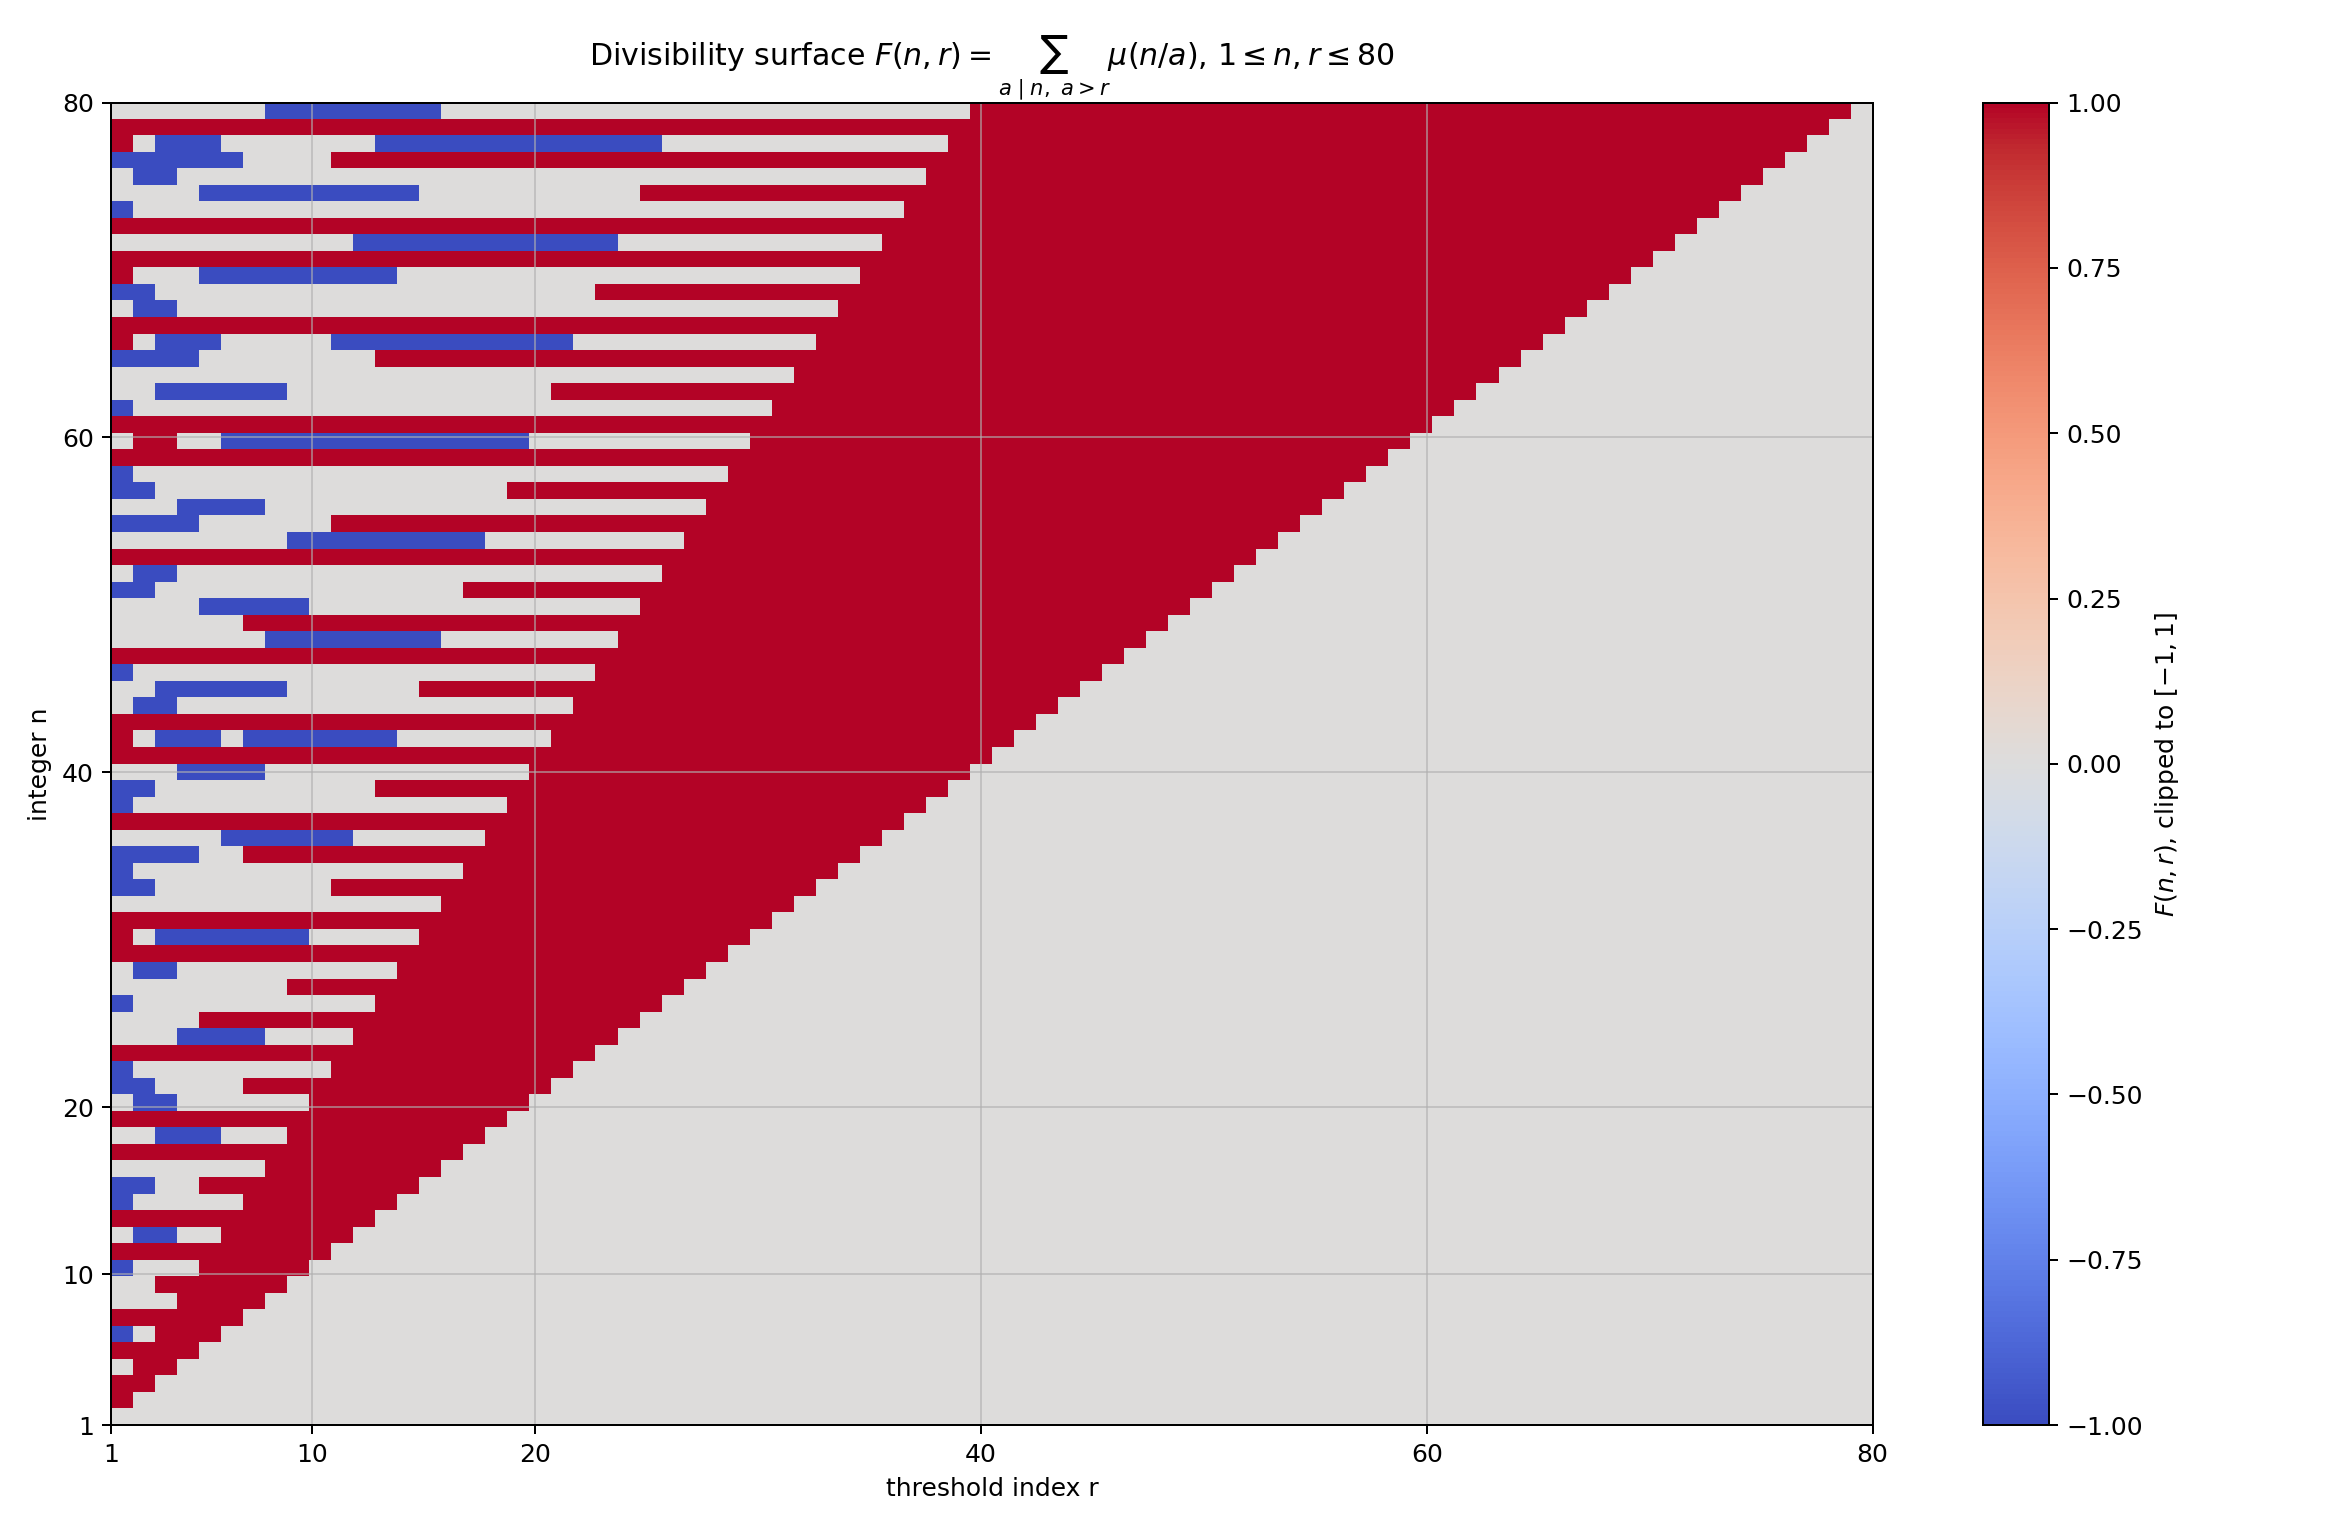
\includegraphics[width=0.96\textwidth]{../figures/mobius_heatmap_N80_en.png}
\caption{Heat map of $F(n,r)$ for $1\le n,r\le80$.  The horizontal coordinate is the threshold $r$ and the vertical coordinate is the integer $n$.  Colors are clipped to $[-1,1]$ only for visualization; the arithmetic values themselves are not truncated.}
\label{fig:mobius_heatmap}
\end{figure}

\begin{figure}[htbp]
\centering
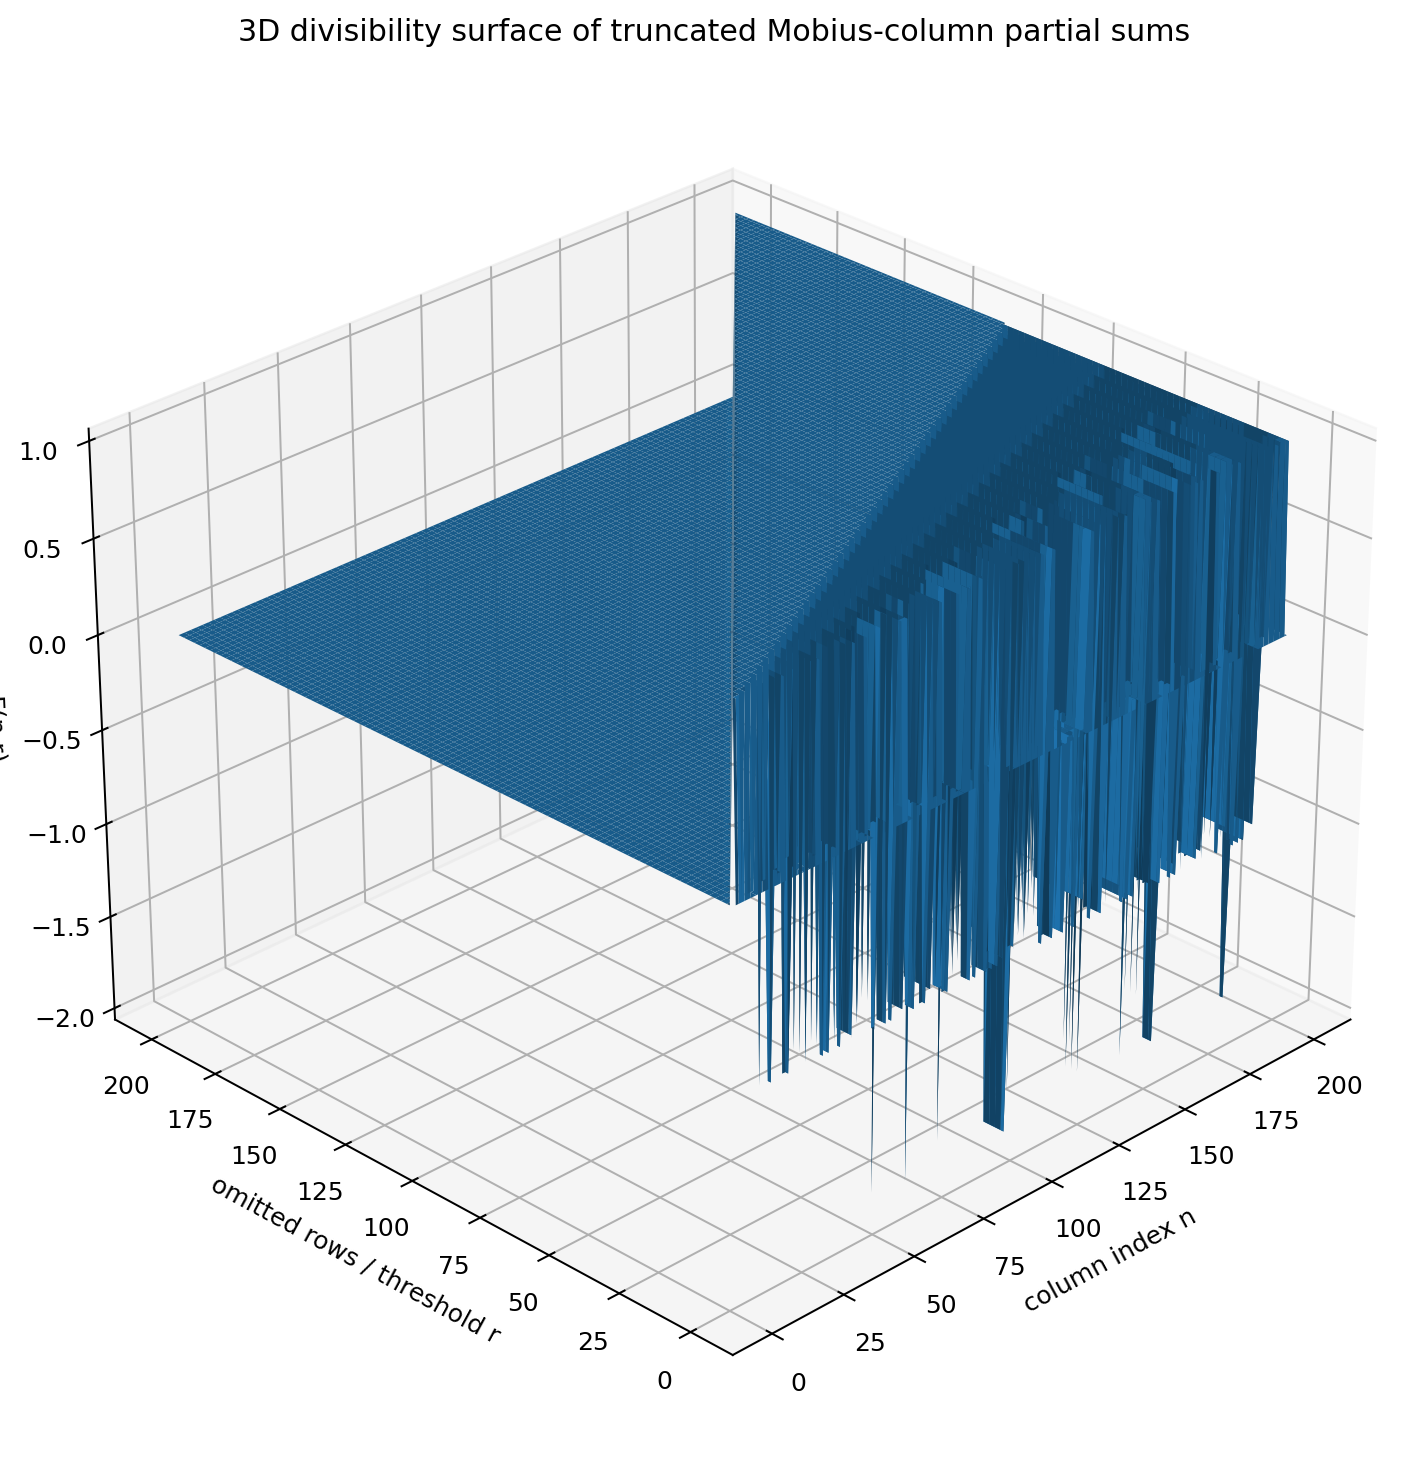
\includegraphics[width=0.96\textwidth]{../figures/mobius_surface_3d_N200_en.png}
\caption{Three-dimensional view of $F(n,r)$ for $1\le n\le200$ and $0\le r\le200$.  The flat region for $r\ge n$ is the exact zero region of the thresholded divisor sum.}
\label{fig:mobius_surface_3d}
\end{figure}


The main structural calculations derived for this particular surface are as follows.
\begin{enumerate}[label=(\roman*)]
\item The full inverse Gram matrix $G_N^{-1}$ is computed entry by entry as a double first difference of $(\tau\circ\gcd)$.  This extends the diagonal computation behind the inverse Frobenius identity to the full off-diagonal kernel.
\item Writing $B_N=KL$, the complementary Gram side is computed through an exact formula for $(K^*K)_{a,b}$ as a signed squarefree--coprime count.  Consequently $G_N=L^*K^*KL$ has a fully explicit finite arithmetic formula.
\item The piecewise-constant structure of $r\mapsto F(n,r)$ gives an exact divisor-gap row-energy identity, with $\varphi(p^k)$ for prime powers and $(p-1)(q+1)$ for semiprimes $pq$, $p<q$.  Combined with the inverse Frobenius identity, this yields the surface-specific condition-number bound $\kappa_2(B_N)\ge(1+o(1))\sqrt{2N\log N}$.
\item In surface coordinates,
\begin{equation}
B_N^{-1}\mob_N=-e_1,
\qquad
B_N^{-1}\liou_N=s_N,
\qquad
s_N(r)=\one_{r+1=\square}-\one_{r=\square},
\label{eq:mu_lambda_coordinate_preview}
\end{equation}
so the Liouville vector becomes the first difference of the square indicator.
\item The local valuation-parity variables are linked exactly to adjacent Liouville correlation by
\begin{equation}
\liou(n)\liou(n+1)=\eta_p(n)h_p(n-1)h_p(n),
\label{eq:intro_eta_lambda_bridge}
\end{equation}
with the dyadic--triadic consequence $\eta_2(n)\eta_3(n)=g(n-1)g(n)$.  These are identities, not independence statements.
\item The determinant-one square-extraction construction is closed branchwise under simultaneous admissible square division and CRT.  The branchwise preservation of determinant one, rather than the classical square-divisor expansion itself, is the structural point isolated here.
\item The intrinsic operator $D_N=(B_NJ_NB_N^{-1}-(B_NJ_NB_N^{-1})^*)/(2i)$ has an exact congruence-divisor kernel depending only on $B_N$ and its canonical factorization $B_N=K_NL_N$, with no zeta input.  An elementary divisor-counting argument gives the unconditional bound $\lambda_{\max}(D_N)=O_\eps(N^{1/2+\eps})$ for every $\eps>0$.  Its upper spectral modes also form numerically persistent branches through $N=131072$, on the empirical scale $\sqrt{N\log N}$, consistent with but sharper than the proven polynomial order.
\end{enumerate}

The intrinsic operator $D_N$ is presented here only as a finite Hermitian construction with an exact arithmetic kernel and a proven unconditional growth bound; no spectral identification with the Riemann zeros, and no Hilbert--Pólya program, is proposed or pursued in this version.

The paper also records several exact consequences whose underlying arithmetic or linear algebra is classical, including the bounded nilpotence of the raw squarefree compression and the associated Jordan bookkeeping.  They are used diagnostically and are not included among the novelty claims above.

\section{Notation and status conventions}
\label{sec:notation}

\begin{center}
\begin{tabular}{>{\raggedright\arraybackslash}p{0.23\textwidth} >{\raggedright\arraybackslash}p{0.65\textwidth}}
\toprule
Symbol & Meaning\\
\midrule
$\mob(n)$ & Möbius function.\\
$\liou(n)$ & Liouville function $(-1)^{\Omega(n)}$.\\
$\Omega(n)$ & Number of prime factors counted with multiplicity.\\
$\omega(n)$ & Number of distinct prime factors.\\
$\Fsurf(n,r)$ & Divisibility surface in \eqref{eq:abstract_surface}.\\
$\Vjump(n,r)$ & Vertical jump in \eqref{eq:vertical_jump_definition}.\\
$B_N$ & Surface matrix on $2\le n\le N$, $1\le r\le N-1$.\\
$G_N$ & Gram matrix $B_N^*B_N$.\\
$S_h$ & Truncated additive shift on the integer coordinate.\\
$T_{N,h}$ & Conjugated shift $B_N^{-1}S_hB_N$.\\
$P_{\mathrm{sf}}$ & Pointwise squarefree projection $f(n)\mapsto\mob(n)^2f(n)$.\\
$Q,R$ & Mutually inverse square-extraction convolution operators; they are not projections.\\
$\what(X)$ & Logarithmic-window parameter, $1\le\what(X)\le X$, $\what(X)\to\infty$.\\
$\zeta(s)$ & Riemann zeta function.\\
$\rho=\beta+i\gamma$ & Generic nontrivial zero of $\zeta$; $\gamma$ is reserved for zero ordinates.\\
\bottomrule
\end{tabular}
\end{center}

Every theorem in the paper is labeled by status in its title or opening sentence.  ``Unconditional'' means that no unproved hypothesis such as RH is assumed; a theorem may still use a previously proved theorem from the literature as an external input, and that input is stated explicitly.  Results that merely rewrite a classical identity are identified as such.

\section{The Möbius divisibility surface}
\label{sec:surface}

\begin{definition}[Divisibility surface]
\label{def:surface}
For $n\ge1$ and integer $r\ge0$, define
\begin{equation}
\Fsurf(n,r)=\sum_{\substack{a\mid n\\a>r}}\mob(n/a).
\label{eq:surface_definition}
\end{equation}
For $r\ge1$ define the vertical jump by
\begin{equation}
\Vjump(n,r)=\Fsurf(n,r-1)-\Fsurf(n,r).
\label{eq:vertical_jump_definition}
\end{equation}
\end{definition}

\begin{lemma}[Vertical jump identity, unconditional]
\label{lem:vertical_jump}
For all integers $n,r\ge1$,
\begin{equation}
\Vjump(n,r)=\one_{r\mid n}\mob(n/r).
\label{eq:vertical_jump_identity}
\end{equation}
\end{lemma}

\begin{proof}
The two finite divisor sums in \eqref{eq:vertical_jump_definition} differ only by the divisor $a=r$.  This divisor occurs exactly when $r\mid n$, and then its contribution is $\mob(n/r)$.
\end{proof}

\subsection{Finite inversion}
\label{subsec:finite_inversion}

\begin{theorem}[Finite inverse, unconditional]
\label{thm:finite_inverse}
Let $N\ge2$ and define $B_N$ by \eqref{eq:BN_intro}.  Then
\begin{equation}
\det B_N=1,
\label{eq:BN_determinant}
\end{equation}
and
\begin{equation}
(B_N^{-1})_{r,n}=\one_{n\mid r+1}-\one_{n\mid r},
\qquad
1\le r\le N-1,\ 2\le n\le N.
\label{eq:BN_inverse}
\end{equation}
Consequently, if
\begin{equation}
y(n)=\sum_{r=1}^{N-1}\Fsurf(n,r)x(r),
\qquad 2\le n\le N,
\label{eq:finite_system}
\end{equation}
then
\begin{equation}
x(r)=
\sum_{\substack{n\mid r+1\\2\le n\le N}}y(n)
-
\sum_{\substack{n\mid r\\2\le n\le N}}y(n).
\label{eq:finite_reconstruction}
\end{equation}
\end{theorem}

\begin{proof}
Define the $(N-1)\times(N-1)$ matrices
\begin{equation}
K_{n,a}=\one_{a\mid n}\mob(n/a),
\qquad 2\le n,a\le N,
\label{eq:K_definition}
\end{equation}
and
\begin{equation}
L_{a,r}=\one_{a>r},
\qquad 2\le a\le N,\ 1\le r\le N-1.
\label{eq:L_definition}
\end{equation}
Then
\begin{equation}
(KL)_{n,r}=\sum_{\substack{a\mid n\\a>r}}\mob(n/a)=\Fsurf(n,r),
\label{eq:BN_factorization}
\end{equation}
so $B_N=KL$.  In increasing order, $K$ is lower triangular with diagonal one.  Its inverse is the finite divisor-zeta matrix
\begin{equation}
(K^{-1})_{a,n}=\one_{n\mid a}.
\label{eq:K_inverse}
\end{equation}
After reindexing $a=i+1$, $L$ is the ordinary lower-triangular summation matrix, whose inverse is the first-difference matrix.  Therefore
\begin{align}
(B_N^{-1})_{r,n}
&=(L^{-1}K^{-1})_{r,n}
\label{eq:BN_inverse_factorized}\\
&=(K^{-1})_{r+1,n}-(K^{-1})_{r,n}
\label{eq:BN_inverse_difference}\\
&=\one_{n\mid r+1}-\one_{n\mid r}.
\label{eq:BN_inverse_final}
\end{align}
Both $K$ and $L$ have determinant one, proving \eqref{eq:BN_determinant}.  Equation \eqref{eq:finite_reconstruction} is $x=B_N^{-1}y$.  All matrices are finite, so there is no convergence or boundary issue.
\end{proof}

\subsection{Exact forward Gram kernel}
\label{subsec:forward_gram_kernel}

For integers $T,m\ge1$ define the squarefree--coprime counting function
\begin{equation}
\mathcal Q_{\mathrm{sf}}(T;m)
=\#\{1\le t\le T:\mob^2(t)=1,\ \gcd(t,m)=1\}.
\label{eq:Qsf_definition}
\end{equation}

\begin{lemma}[Finite inclusion--exclusion for $\mathcal Q_{\mathrm{sf}}$; standard]
\label{lem:Qsf_inclusion_exclusion}
For every $T,m\ge1$,
\begin{equation}
\mathcal Q_{\mathrm{sf}}(T;m)
=\sum_{\substack{d\le\sqrt T\\(d,m)=1}}\mob(d)
\sum_{e\mid m}\mob(e)
\left\lfloor\frac{T}{d^2e}\right\rfloor.
\label{eq:Qsf_inclusion_exclusion}
\end{equation}
This is the standard finite inclusion--exclusion for squarefreeness and coprimality and is not claimed as new.
\end{lemma}

\begin{proof}
Use
\begin{equation}
\mob^2(t)=\sum_{d^2\mid t}\mob(d),
\qquad
\one_{(t,m)=1}=\sum_{e\mid(t,m)}\mob(e),
\label{eq:Qsf_indicators}
\end{equation}
and interchange finite sums.  If $d^2\mid t$ and $(t,m)=1$, necessarily $(d,m)=1$; writing $t=d^2s$, the remaining condition is $(s,m)=1$, whose finite inclusion--exclusion gives the inner sum in \eqref{eq:Qsf_inclusion_exclusion}.
\end{proof}

\begin{theorem}[Exact $K^*K$ squarefree--coprime kernel, unconditional]
\label{thm:KstarK_kernel}
Let $2\le a,b\le N$, put
\begin{equation}
g=\gcd(a,b),
\qquad a'=a/g,
\qquad b'=b/g,
\qquad T=\left\lfloor\frac{N}{\lcm(a,b)}\right\rfloor.
\label{eq:KstarK_reduced_parameters}
\end{equation}
Then
\begin{equation}
(K^*K)_{a,b}=
\begin{cases}
\mob(a')\mob(b')\,\mathcal Q_{\mathrm{sf}}(T;a'b'),
& a',b'\text{ squarefree},\\[4pt]
0,&\text{otherwise}.
\end{cases}
\label{eq:KstarK_exact}
\end{equation}
\end{theorem}

\begin{proof}
By \eqref{eq:K_definition},
\begin{equation}
(K^*K)_{a,b}
=\sum_{\substack{n\le N\\a\mid n,\ b\mid n}}
\mob(n/a)\mob(n/b).
\label{eq:KstarK_start}
\end{equation}
Write $n=\lcm(a,b)t=ga'b't$.  Then
\begin{equation}
n/a=b't,
\qquad n/b=a't,
\label{eq:KstarK_quotients}
\end{equation}
so
\begin{equation}
(K^*K)_{a,b}=\sum_{1\le t\le T}\mob(b't)\mob(a't).
\label{eq:KstarK_tsum}
\end{equation}
If either $a'$ or $b'$ is not squarefree, every summand is zero.  Otherwise $(a',b')=1$, and a summand is nonzero exactly when $t$ is squarefree and $(t,a'b')=1$.  On those terms complete multiplicativity on coprime arguments gives
\begin{equation}
\mob(a't)\mob(b't)
=\mob(a')\mob(b')\mob(t)^2
=\mob(a')\mob(b').
\label{eq:KstarK_sign_collapse}
\end{equation}
Counting the surviving $t$ proves \eqref{eq:KstarK_exact}.
\end{proof}

\begin{corollary}[Exact full Gram matrix, unconditional]
\label{cor:full_gram_exact}
For $1\le r,q\le N-1$,
\begin{equation}
G_N(r,q)
=\sum_{a=r+1}^{N}\sum_{b=q+1}^{N}(K^*K)_{a,b},
\label{eq:full_gram_from_K}
\end{equation}
where every term on the right is given explicitly by \eqref{eq:KstarK_exact} and \eqref{eq:Qsf_inclusion_exclusion}.
\end{corollary}

\begin{proof}
Since $B_N=KL$,
\begin{equation}
G_N=B_N^*B_N=L^*K^*KL.
\label{eq:G_LKL}
\end{equation}
Using $L_{a,r}=\one_{a>r}$ gives \eqref{eq:full_gram_from_K}.
\end{proof}

\begin{remark}[Status of the forward Gram formula]
\label{rem:forward_gram_status}
Formula \eqref{eq:Qsf_inclusion_exclusion} is standard inclusion--exclusion, and general gcd/incidence matrix factorizations are classical.  The content derived here is the specialization of the particular Möbius incidence factor $K$ from \eqref{eq:K_definition} to the exact kernel \eqref{eq:KstarK_exact}, and its consequent explicit reconstruction of the surface Gram matrix through \eqref{eq:full_gram_from_K}.  No claim of priority is made for the general background on gcd matrices.
\end{remark}

\begin{corollary}[Biorthogonality, unconditional]
\label{cor:biorthogonality}
For $1\le r,q\le N-1$,
\begin{equation}
\sum_{n=2}^{N}
\bigl(\one_{n\mid r+1}-\one_{n\mid r}\bigr)\Fsurf(n,q)
=\delta_{rq}.
\label{eq:biorthogonality}
\end{equation}
\end{corollary}

\begin{proof}
This is the $(r,q)$ entry of $B_N^{-1}B_N=I$.
\end{proof}

\subsection{Frobenius identity}
\label{subsec:frobenius}

\begin{proposition}[Exact Frobenius identity, unconditional]
\label{prop:frobenius}
Let $\sigma_1,\ldots,\sigma_{N-1}$ be the singular values of $B_N$, and let
\begin{equation}
\TauSum(N)=\sum_{m\le N}\tau(m).
\label{eq:tau_summatory}
\end{equation}
Then
\begin{equation}
\prod_{j=1}^{N-1}\sigma_j=1
\label{eq:singular_product}
\end{equation}
and
\begin{equation}
\sum_{j=1}^{N-1}\sigma_j^{-2}
=2\TauSum(N)-\tau(N)-2N+1.
\label{eq:frobenius_identity}
\end{equation}
\end{proposition}

\begin{proof}
The first identity is $|\det B_N|=1$.  By \eqref{eq:BN_inverse}, row $r$ of $B_N^{-1}$ contains disjoint indicators of divisors $n\ge2$ of $r+1$ and $r$; they cannot overlap because a common $n\ge2$ would divide $1$.  Hence
\begin{equation}
\sum_{n=2}^{N}|(B_N^{-1})_{r,n}|^2
=\tau(r+1)+\tau(r)-2.
\label{eq:inverse_row_norm}
\end{equation}
Summing over $1\le r\le N-1$ yields \eqref{eq:frobenius_identity}, because the singular values of $B_N^{-1}$ are $\sigma_j^{-1}$.
\end{proof}

\begin{theorem}[Exact surface row-energy identity, unconditional]
\label{thm:surface_row_energy}
Fix $n>1$ and list its positive divisors as
\begin{equation}
1=d_1<d_2<\cdots<d_k=n,
\qquad d_0:=0,
\label{eq:ordered_divisors_row}
\end{equation}
where $k=\tau(n)$.  Define the partial Möbius sums on the ordered divisor set by
\begin{equation}
M_n(j)=\sum_{i=1}^{j}\mob(d_i),
\qquad 1\le j\le k.
\label{eq:Mn_divisor_partial}
\end{equation}
Then
\begin{equation}
\sum_{r=0}^{n}\Fsurf(n,r)^2
=\sum_{i=0}^{k-1}(d_{i+1}-d_i)\,M_n(k-i)^2.
\label{eq:surface_row_energy}
\end{equation}
Since $\Fsurf(n,0)=\Fsurf(n,n)=0$ for $n>1$ and $\Fsurf(n,r)=0$ for $r\ge n$, the same quantity is the squared Euclidean norm of the $n$th row of $B_N$ whenever $n\le N$.
\end{theorem}

\begin{proof}
If $d_i\le r<d_{i+1}$, then the divisors $a\mid n$ satisfying $a>r$ are $d_{i+1},\ldots,d_k$.  Under the order-reversing bijection $a\mapsto n/a$, their quotients are $d_1,\ldots,d_{k-i}$.  Hence
\begin{equation}
\Fsurf(n,r)=M_n(k-i)
\qquad(d_i\le r<d_{i+1}).
\label{eq:F_piecewise_Mn}
\end{equation}
There are exactly $d_{i+1}-d_i$ integer values of $r$ in this half-open interval.  Summing the constant square on each interval proves \eqref{eq:surface_row_energy}.  Finally $\Fsurf(n,0)=\sum_{d\mid n}\mob(d)=0$ for $n>1$, while $\Fsurf(n,r)=0$ for $r\ge n$.
\end{proof}

\begin{corollary}[Prime-power and semiprime row energies]
\label{cor:row_energy_special_cases}
For every prime $p$ and integer $a\ge1$,
\begin{equation}
\sum_r\Fsurf(p^a,r)^2=\varphi(p^a).
\label{eq:prime_power_row_energy}
\end{equation}
If $p<q$ are distinct primes, then
\begin{equation}
\sum_r\Fsurf(pq,r)^2=(p-1)(q+1).
\label{eq:semiprime_row_energy}
\end{equation}
Here the sums may be taken over $0\le r\le n$ or over the corresponding row of any $B_N$ with $N\ge n$.
\end{corollary}

\begin{proof}
For $n=p^a$, the ordered Möbius values on the divisors are $1,-1,0,\ldots,0$, so all partial sums except $M_n(1)=1$ vanish; the surviving interval has length $p^a-p^{a-1}=\varphi(p^a)$.  For $n=pq$ with $p<q$, the ordered divisors are $1,p,q,pq$ and the partial sums are $1,0,-1,0$.  Formula \eqref{eq:surface_row_energy} therefore gives
\begin{equation}
(p-1)+q(p-1)=(p-1)(q+1).
\end{equation}
\end{proof}

\begin{corollary}[Forward Frobenius identity in divisor-gap form]
\label{cor:forward_frobenius}
With the notation of Theorem \ref{thm:surface_row_energy},
\begin{equation}
\sum_{j=1}^{N-1}\sigma_j^2
=\|B_N\|_F^2
=\sum_{n=2}^{N}\sum_{i=0}^{\tau(n)-1}
(d_{i+1}-d_i)M_n(\tau(n)-i)^2.
\label{eq:forward_frobenius_gap}
\end{equation}
\end{corollary}

\begin{proof}
Sum \eqref{eq:surface_row_energy} over the rows $2\le n\le N$ and use the standard identity $\|B_N\|_F^2=\sum_j\sigma_j^2$.
\end{proof}

\begin{theorem}[Exact inverse Gram--gcd identity, unconditional]
\label{thm:inverse_gram_gcd}
Let $G_N=B_N^*B_N$.  For $1\le r,q\le N-1$,
\begin{align}
(G_N^{-1})_{r,q}
={}&\tau\bigl(\gcd(r+1,q+1)\bigr)
-\tau\bigl(\gcd(r+1,q)\bigr) \notag\\
&-\tau\bigl(\gcd(r,q+1)\bigr)
+\tau\bigl(\gcd(r,q)\bigr).
\label{eq:inverse_gram_gcd}
\end{align}
Consequently $G_N^{-1}$ is an integral symmetric positive-definite matrix with determinant one.  Here ``positive-definite'' means
\begin{equation}
x^*G_N^{-1}x>0\qquad(x\ne0);
\label{eq:inverse_gram_positive_definite}
\end{equation}
no entrywise positivity is asserted.
\end{theorem}

\begin{proof}
Since $G_N=B_N^*B_N$,
\begin{equation}
G_N^{-1}=B_N^{-1}(B_N^{-1})^*.
\label{eq:inverse_gram_factorization}
\end{equation}
Using \eqref{eq:BN_inverse},
\begin{align}
(G_N^{-1})_{r,q}
={}&\sum_{n=2}^{N}
\bigl(\one_{n\mid r+1}-\one_{n\mid r}\bigr)
\bigl(\one_{n\mid q+1}-\one_{n\mid q}\bigr).
\label{eq:inverse_gram_indicator_sum}
\end{align}
For $a,b\le N$,
\begin{equation}
\sum_{n=2}^{N}\one_{n\mid a}\one_{n\mid b}
=\tau(\gcd(a,b))-1.
\label{eq:common_divisor_count}
\end{equation}
Expanding \eqref{eq:inverse_gram_indicator_sum} gives four expressions of the form \eqref{eq:common_divisor_count}; their constant $-1$ terms cancel, proving \eqref{eq:inverse_gram_gcd}.  Integrality and symmetry are immediate.  Positive definiteness follows from \eqref{eq:inverse_gram_factorization} and invertibility of $B_N$, while
$\det G_N^{-1}=|\det B_N|^{-2}=1$.
\end{proof}

\begin{remark}[Sign pattern]
\label{rem:inverse_gram_sign}
The positivity in Theorem \ref{thm:inverse_gram_gcd} is quadratic-form positivity, not entrywise positivity.  For example,
\begin{equation}
(G_N^{-1})_{1,2}=1-2-1+1=-1
\qquad(N\ge3).
\label{eq:inverse_gram_negative_entry}
\end{equation}
Thus the content is the exact arithmetic formula for the full inverse Gram kernel; positive definiteness itself is automatic for the inverse of a positive-definite Gram matrix.
\end{remark}

\begin{corollary}[Quantitative anisotropy from the two Frobenius sides]
\label{cor:condition_number_growth}
Let $P(N)$ denote the largest prime not exceeding $N$.  Then, for $N\ge2$,
\begin{equation}
\kappa_2(B_N)^2
\ge
(P(N)-1)\,
\frac{2\TauSum(N)-\tau(N)-2N+1}{N-1}.
\label{eq:condition_number_exact_lower}
\end{equation}
Consequently,
\begin{equation}
\kappa_2(B_N)
\ge (1+o(1))\sqrt{2N\log N}.
\label{eq:condition_number_lower}
\end{equation}
\end{corollary}

\begin{proof}
By \eqref{eq:prime_power_row_energy}, the row of $B_N$ indexed by the prime $P(N)$ has squared Euclidean norm $P(N)-1$.  Since every row norm is bounded above by the spectral norm,
\begin{equation}
\sigma_{\max}(B_N)^2\ge P(N)-1.
\label{eq:sigma_max_prime_row}
\end{equation}
On the inverse side, Proposition \ref{prop:frobenius} gives
\begin{equation}
\sigma_{\min}(B_N)^{-2}
=\max_j\sigma_j^{-2}
\ge
\frac{2\TauSum(N)-\tau(N)-2N+1}{N-1}.
\label{eq:sigma_min_inverse_average}
\end{equation}
Multiplying \eqref{eq:sigma_max_prime_row} and \eqref{eq:sigma_min_inverse_average} proves \eqref{eq:condition_number_exact_lower}.  The classical estimates
\begin{equation}
P(N)=N(1+o(1)),
\qquad
\TauSum(N)=N\log N+(2\gamma_{\mathrm E}-1)N+O(\sqrt N)
\label{eq:classical_prime_divisor_asymptotics}
\end{equation}
then give \eqref{eq:condition_number_lower}.
\end{proof}

\begin{remark}[Status of Corollary \ref{cor:condition_number_growth}]
The row identity \eqref{eq:prime_power_row_energy} and the exact inverse Frobenius identity are properties of the present surface matrix.  The asymptotics in \eqref{eq:classical_prime_divisor_asymptotics} are classical.  Thus \eqref{eq:condition_number_exact_lower} is an exact matrix consequence and \eqref{eq:condition_number_lower} is its classical-asymptotic corollary; no new prime-distribution or divisor-problem estimate is claimed.
\end{remark}

\section{Difference--convolution intertwining}
\label{sec:intertwining}

For arithmetic functions $f,g$, use the convention
\begin{equation}
(f*g)(n)=\sum_{a\mid n}f(n/a)g(a).
\label{eq:dirichlet_convolution}
\end{equation}

\begin{theorem}[Difference--convolution intertwining, unconditional]
\label{thm:intertwining}
For any arithmetic function $g$ and every $n>1$,
\begin{equation}
(\mob*g)(n)=\sum_{r=1}^{n-1}\Fsurf(n,r)\bigl(g(r+1)-g(r)\bigr).
\label{eq:intertwining}
\end{equation}
\end{theorem}

\begin{proof}
All sums are finite.  Interchanging them gives
\begin{align}
\sum_{r=1}^{n-1}\Fsurf(n,r)(g(r+1)-g(r))
&=\sum_{a\mid n}\mob(n/a)\sum_{r=1}^{a-1}(g(r+1)-g(r))
\label{eq:intertwining_swap}\\
&=\sum_{a\mid n}\mob(n/a)(g(a)-g(1))
\label{eq:intertwining_telescope}\\
&=(\mob*g)(n)-g(1)\sum_{a\mid n}\mob(n/a).
\label{eq:intertwining_last}
\end{align}
The last divisor sum is zero for $n>1$.
\end{proof}

\begin{corollary}[Universal finite reconstruction, unconditional]
\label{cor:universal_reconstruction}
Let $f:\N\to\C$ and define
\begin{equation}
G_f(m)=\sum_{d\mid m}f(d).
\label{eq:Gf_definition}
\end{equation}
Then for $n>1$,
\begin{equation}
f(n)=\sum_{r=1}^{n-1}\Fsurf(n,r)\bigl(G_f(r+1)-G_f(r)\bigr).
\label{eq:universal_reconstruction}
\end{equation}
\end{corollary}

\begin{proof}
Classical Möbius inversion gives $f=\mob*G_f$.  Apply Theorem \ref{thm:intertwining}.
\end{proof}

\section{Dirichlet transforms and Mellin domain}
\label{sec:analytic_transforms}

This section records the analytic transforms that are needed later and states their domains explicitly; the underlying Dirichlet-series manipulations are classical, see \cite{Apostol1976}.  No contour shift is used to deduce any arithmetic theorem in this paper.

\begin{definition}[Double zeta tail]
\label{def:zeta2}
For $\Re s>1$ and $\Re w>1$, define
\begin{equation}
\zeta_2(s,w)=\sum_{a>r\ge1}a^{-s}r^{-w}.
\label{eq:zeta2_definition}
\end{equation}
The series converges absolutely and locally uniformly in that product half-plane and is therefore holomorphic there.
\end{definition}

\begin{proposition}[Surface transform, unconditional]
\label{prop:surface_transform}
If $\Re s>1$ and $\Re w>1$, then
\begin{equation}
\mathscr F(s,w)
:=\sum_{n,r\ge1}\frac{\Fsurf(n,r)}{n^s r^w}
=\frac{\zeta_2(s,w)}{\zeta(s)}.
\label{eq:surface_transform}
\end{equation}
Both sides are holomorphic in this domain.
\end{proposition}

\begin{proof}
Put $\sigma=\Re s$ and $\tau=\Re w$.  Absolute convergence follows from
\begin{align}
\sum_{r\ge1}\sum_{a>r}\sum_{m\ge1}
\frac{|\mob(m)|}{(am)^\sigma r^\tau}
&\le \zeta(\sigma)\sum_{a,r\ge1}\frac1{a^\sigma r^\tau}
\label{eq:surface_absolute_bound}\\
&=\zeta(\sigma)^2\zeta(\tau)<\infty.
\label{eq:surface_absolute_bound_final}
\end{align}
Tonelli's theorem therefore justifies the rearrangement of absolute values, and Fubini's theorem justifies the rearrangement of the original series.  Writing $n=am$ gives
\begin{align}
\mathscr F(s,w)
&=\sum_{r\ge1}\sum_{a>r}\sum_{m\ge1}
\frac{\mob(m)}{(am)^s r^w}
\label{eq:surface_transform_expand}\\
&=\left(\sum_{m\ge1}\frac{\mob(m)}{m^s}\right)
\sum_{a>r\ge1}\frac1{a^s r^w}
\label{eq:surface_transform_factor}\\
&=\frac{\zeta_2(s,w)}{\zeta(s)}.
\label{eq:surface_transform_finish}
\end{align}
Since $\zeta(s)$ has no zeros for $\Re s>1$, the quotient is holomorphic there.  Local uniform convergence supplies the same conclusion directly for the defining series.
\end{proof}

\begin{proposition}[Jump transform, unconditional]
\label{prop:jump_transform}
If
\begin{equation}
\Re s>1,
\qquad
\Re(s+w)>1,
\label{eq:jump_transform_domain}
\end{equation}
then
\begin{equation}
\mathscr V(s,w)
:=\sum_{n,r\ge1}\frac{\Vjump(n,r)}{n^s r^w}
=\frac{\zeta(s+w)}{\zeta(s)}.
\label{eq:jump_transform}
\end{equation}
The defining double series converges absolutely and locally uniformly on compact subsets of \eqref{eq:jump_transform_domain}; hence it is holomorphic there.
\end{proposition}

\begin{proof}
Using Lemma \ref{lem:vertical_jump}, put $n=rm$.  For $\sigma=\Re s$ and $\upsilon=\Re(s+w)$,
\begin{equation}
\sum_{r,m\ge1}\frac{|\mob(m)|}{m^\sigma r^\upsilon}
\le \zeta(\sigma)\zeta(\upsilon)<\infty.
\label{eq:jump_absolute_bound}
\end{equation}
Thus
\begin{align}
\mathscr V(s,w)
&=\sum_{r,m\ge1}\frac{\mob(m)}{m^s r^{s+w}}
\label{eq:jump_transform_expand}\\
&=\left(\sum_{m\ge1}\frac{\mob(m)}{m^s}\right)
\left(\sum_{r\ge1}\frac1{r^{s+w}}\right)
\label{eq:jump_transform_factor}\\
&=\frac{\zeta(s+w)}{\zeta(s)}.
\label{eq:jump_transform_finish}
\end{align}
The same absolute bounds are uniform on compact subsets separated from the boundary of the two half-planes, proving local uniform convergence and holomorphy.
\end{proof}

\begin{definition}[One-parameter jump family]
\label{def:Aw}
For $w\in\C$ and $n\ge1$, define the finite divisor sum
\begin{equation}
A_w(n)=\sum_{r\mid n}\mob(n/r)r^{-w}.
\label{eq:Aw_definition}
\end{equation}
For each fixed $n$, $w\mapsto A_w(n)$ is an entire function.
\end{definition}

\begin{proposition}[Dirichlet series and logarithmic derivatives, unconditional]
\label{prop:Aw}
In the domain \eqref{eq:jump_transform_domain},
\begin{equation}
\sum_{n\ge1}\frac{A_w(n)}{n^s}=\frac{\zeta(s+w)}{\zeta(s)}.
\label{eq:Aw_dirichlet}
\end{equation}
For $k\ge0$, define
\begin{equation}
\operatorname{Mang}_k(n)=\sum_{r\mid n}\mob(n/r)(\log r)^k.
\label{eq:Mang_definition}
\end{equation}
Then, for each fixed $n$,
\begin{equation}
\operatorname{Mang}_k(n)
=(-1)^k\left.\frac{\partial^k}{\partial w^k}A_w(n)\right|_{w=0},
\label{eq:Mang_from_Aw}
\end{equation}
and for $\Re s>1$,
\begin{equation}
\sum_{n\ge1}\frac{\operatorname{Mang}_k(n)}{n^s}
=(-1)^k\frac{\zeta^{(k)}(s)}{\zeta(s)}.
\label{eq:Mang_dirichlet}
\end{equation}
In particular $\operatorname{Mang}_1$ is the usual von Mangoldt function.
\end{proposition}

\begin{proof}
Equation \eqref{eq:Aw_dirichlet} is Proposition \ref{prop:jump_transform} with the $r$-sum performed first.  Equation \eqref{eq:Mang_from_Aw} is differentiation of a finite divisor sum and requires no convergence argument.  To justify differentiation of \eqref{eq:Aw_dirichlet}, fix $\Re s>1$ and choose $\delta>0$ such that $\Re s-\delta>1$.  For $|w|\le\delta/2$ the double series for $\zeta(s+w)/\zeta(s)$ and all $w$-derivatives up to any fixed order are dominated by
\begin{equation}
\sum_{r,m\ge1}\frac{(\log r)^k}{m^{\Re s}r^{\Re s-\delta/2}},
\label{eq:Aw_derivative_domination}
\end{equation}
which converges.  Uniform convergence on the closed disk permits termwise differentiation by the Weierstrass theorem.  Evaluating at $w=0$ gives \eqref{eq:Mang_dirichlet}.
\end{proof}

\begin{proposition}[Mellin representation, unconditional in its domain]
\label{prop:mellin}
Let $h\in C_c^\infty(0,\infty)$ and define
\begin{equation}
\widehat h(s)=\int_0^\infty h(x)x^{s-1}\,dx.
\label{eq:mellin_transform}
\end{equation}
Let $c\in\R$ satisfy
\begin{equation}
c>1,
\qquad
\Re(c+w)>1.
\label{eq:mellin_domain}
\end{equation}
Then for $X>0$,
\begin{equation}
\sum_{n\ge1}A_w(n)h(n/X)
=\frac1{2\pi i}\int_{c-i\infty}^{c+i\infty}
\frac{\zeta(s+w)}{\zeta(s)}\widehat h(s)X^s\,ds.
\label{eq:mellin_representation}
\end{equation}
The integral is absolutely convergent.
\end{proposition}

\begin{proof}
For $h\in C_c^\infty(0,\infty)$, $\widehat h$ is entire and, on every fixed vertical line, decays faster than any inverse power of $|\Im s|$.  Mellin inversion gives
\begin{equation}
h(n/X)=\frac1{2\pi i}\int_{c-i\infty}^{c+i\infty}\widehat h(s)X^s n^{-s}\,ds.
\label{eq:mellin_inversion}
\end{equation}
On $\Re s=c$, Proposition \ref{prop:Aw} gives absolute convergence of $\sum_n A_w(n)n^{-s}$ under \eqref{eq:mellin_domain}.  More explicitly, the absolute majorant is bounded by
\begin{equation}
\sum_{r,m\ge1}\frac1{m^c r^{c+\Re w}}<\infty.
\label{eq:mellin_series_majorant}
\end{equation}
Multiplying this finite bound by the integrable function $|\widehat h(c+it)|X^c$ justifies interchange of the series and the vertical integral by Fubini.  Substitution of \eqref{eq:Aw_dirichlet} proves \eqref{eq:mellin_representation}.
\end{proof}

\begin{remark}[Contour shifts]
\label{rem:contour_shifts}
No contour shift is needed in the arguments of this paper.  If one shifts the line in \eqref{eq:mellin_representation}, a rigorous residue formula must account for the pole of $\zeta(s+w)$ at $s=1-w$, the trivial and nontrivial zeros of the denominator, possible numerator-denominator cancellations, multiple zeros, horizontal contour estimates, and the convergence prescription for the resulting zero sum.  At $w=0$ the quotient is identically one after removable singularities are canceled; one must cancel first and differentiate only afterward if derivatives in $w$ are intended.
\end{remark}

\section{Exact \texorpdfstring{$p$}{p}-adic valuation-parity shells}
\label{sec:padic_shells}

Fix a prime $p$.  Let $m_p$ denote normalized Haar probability measure on the compact additive group $\Z_p$.  The valuation $v_p$ is finite away from $0$; values assigned at finitely many singular points do not affect integrals.

\begin{definition}[Adjacent valuation-parity sign]
\label{def:eta_p}
For $x\in\Z_p\setminus\{0,-1\}$, define
\begin{equation}
\eta_p(x)=(-1)^{v_p(x)+v_p(x+1)}.
\label{eq:eta_p}
\end{equation}
Assign arbitrary values to $\eta_p(0)$ and $\eta_p(-1)$; these two points have Haar measure zero and do not affect any integral or conditional expectation below.  Let $\mathcal F_j$ be the finite $\sigma$-algebra generated by residue classes modulo $p^j$, with $\mathcal F_0$ trivial.  Put
\begin{equation}
M_j=\E(\eta_p\mid\mathcal F_j),
\qquad
\Delta_j=M_j-M_{j-1}\quad(j\ge1).
\label{eq:padic_martingale}
\end{equation}
\end{definition}

\begin{lemma}[Conditional valuation sign, unconditional]
\label{lem:conditional_valuation}
Conditioned on $p\mid x$,
\begin{equation}
\Prob\bigl(v_p(x)=k\mid p\mid x\bigr)=(p-1)p^{-k},
\qquad k\ge1,
\label{eq:valuation_distribution}
\end{equation}
and
\begin{equation}
\E\bigl((-1)^{v_p(x)}\mid p\mid x\bigr)
=-\frac{p-1}{p+1}.
\label{eq:conditional_valuation_mean}
\end{equation}
\end{lemma}

\begin{proof}
The shell $p^k\Z_p\setminus p^{k+1}\Z_p$ has Haar measure $(p-1)p^{-k-1}$.  Division by $m_p(p\Z_p)=p^{-1}$ yields \eqref{eq:valuation_distribution}.  The absolutely convergent geometric series then gives
\begin{equation}
(p-1)\sum_{k\ge1}\frac{(-1)^k}{p^k}=-\frac{p-1}{p+1}.
\label{eq:conditional_valuation_series}
\end{equation}
\end{proof}

\begin{proposition}[Mean and first shell, unconditional]
\label{prop:padic_mean_first_shell}
The Haar mean is
\begin{equation}
M_0=\int_{\Z_p}\eta_p\,dm_p=\frac{p-3}{p+1}.
\label{eq:padic_global_mean}
\end{equation}
On the classes $0,-1\pmod p$, $\Delta_1$ equals
\begin{equation}
-\frac{2(p-2)}{p+1},
\label{eq:first_shell_exceptional}
\end{equation}
and on each of the other $p-2$ classes it equals
\begin{equation}
\frac4{p+1}.
\label{eq:first_shell_ordinary}
\end{equation}
Its energy is
\begin{equation}
\|\Delta_1\|_2^2=\frac{8(p-2)}{(p+1)^2}.
\label{eq:first_shell_energy}
\end{equation}
\end{proposition}

\begin{proof}
On the two exceptional classes the conditional mean is $-(p-1)/(p+1)$ by Lemma \ref{lem:conditional_valuation}; on the remaining classes both valuations vanish, so the value is one.  Averaging over the $p$ classes gives \eqref{eq:padic_global_mean}.  Subtracting this mean gives \eqref{eq:first_shell_exceptional} and \eqref{eq:first_shell_ordinary}; squaring and averaging gives \eqref{eq:first_shell_energy}.
\end{proof}

\begin{corollary}[The unique centered prime, unconditional]
\label{cor:unique_centered_prime}
Among primes,
\begin{equation}
\int_{\Z_p}\eta_p\,dm_p=0
\quad\Longleftrightarrow\quad
p=3.
\label{eq:unique_centered_prime}
\end{equation}
Thus the dyadic local factor has mean $-1/3$, the triadic factor is centered, and every $p>3$ factor has positive mean.
\end{corollary}

\begin{proof}
This is immediate from \eqref{eq:padic_global_mean}.
\end{proof}

\begin{theorem}[Exact martingale shells, unconditional]
\label{thm:exact_shells}
For every $j\ge2$, $\Delta_j$ vanishes outside the two parent classes
\begin{equation}
x\equiv0,-1\pmod{p^{j-1}}.
\label{eq:active_parents}
\end{equation}
On each active parent, its $p$ child values are a permutation of
\begin{equation}
\frac{2(-1)^{j-1}}{p+1}\bigl(-(p-1),1,\ldots,1\bigr).
\label{eq:shell_child_values}
\end{equation}
Consequently,
\begin{equation}
\|\Delta_j\|_2^2
=\frac{8(p-1)}{(p+1)^2}p^{1-j},
\qquad j\ge2,
\label{eq:shell_energy}
\end{equation}
and for $J\ge1$,
\begin{equation}
\sum_{j>J}\|\Delta_j\|_2^2
=\frac{8p^{1-J}}{(p+1)^2}.
\label{eq:shell_tail_energy}
\end{equation}
\end{theorem}

\begin{proof}
On the parent $x\equiv0\pmod{p^{j-1}}$, the conditional mean is
\begin{equation}
(-1)^{j-1}\frac{p-1}{p+1}.
\label{eq:parent_mean_shell}
\end{equation}
The exceptional child $x\equiv0\pmod{p^j}$ has conditional mean with the opposite sign, while each other child has exact valuation $j-1$.  Subtracting the parent mean gives exactly the vector in \eqref{eq:shell_child_values}.  The tower above $-1$ is obtained by $x\mapsto-1-x$ and has the same child multiset.

Each active parent has measure $p^{1-j}$.  The mean square of the child vector within one parent is
\begin{equation}
\frac1p\left(
\frac{4(p-1)^2}{(p+1)^2}
+(p-1)\frac4{(p+1)^2}
\right)
=\frac{4(p-1)}{(p+1)^2}.
\label{eq:child_mean_square}
\end{equation}
Multiplication by the total measure $2p^{1-j}$ gives \eqref{eq:shell_energy}.  Summing the geometric tail gives \eqref{eq:shell_tail_energy}.
\end{proof}

\begin{corollary}[Exact $L^2$ closure and triadic specialization, unconditional]
\label{cor:padic_closure}
The martingale differences are pairwise orthogonal and
\begin{equation}
M_0^2+\sum_{j\ge1}\|\Delta_j\|_2^2=1.
\label{eq:energy_closure}
\end{equation}
For $p=3$,
\begin{equation}
\Delta_1=(-1/2,1,-1/2)
\label{eq:triadic_first_shell}
\end{equation}
on classes $0,1,2\pmod3$,
\begin{equation}
\|\Delta_1\|_2^2=\frac12,
\qquad
\|\Delta_j\|_2^2=3^{1-j}\quad(j\ge2),
\label{eq:triadic_shell_energies}
\end{equation}
and all unit energy lies in the centered nonconstant shells.
\end{corollary}

\begin{proof}
Since conditional expectations onto nested finite $\sigma$-algebras form an $L^2$ martingale, the differences are orthogonal.  The $\sigma$-algebras generated by all residue classes modulo $p^j$ generate the Borel $\sigma$-algebra of $\Z_p$; by the standard $L^2$ martingale convergence theorem, $M_J\to\eta_p$ in $L^2$.  As $|\eta_p|=1$ almost everywhere, Pythagoras gives \eqref{eq:energy_closure}.  The triadic formulas follow by substituting $p=3$ into Proposition \ref{prop:padic_mean_first_shell} and Theorem \ref{thm:exact_shells}.
\end{proof}

\section{Two-shift collision depth and determinant-one geometry}
\label{sec:two_shift}

\begin{definition}[Shifted local parity]
\label{def:eta_ph}
For a prime $p$ and nonzero integer $h$, define
\begin{equation}
\eta_{p,h}(x)=(-1)^{v_p(x)+v_p(x+h)},
\qquad x\in\Z_p\setminus\{0,-h\}.
\label{eq:eta_ph}
\end{equation}
Assign arbitrary values at $0$ and $-h$; they form a Haar-null set.
\end{definition}

\begin{theorem}[Exact two-shift mean, unconditional]
\label{thm:two_shift_mean}
Write
\begin{equation}
h=p^s u,
\qquad s=v_p(h),
\qquad p\nmid u.
\label{eq:h_factorization}
\end{equation}
Then
\begin{equation}
\int_{\Z_p}\eta_{p,h}(x)\,dm_p(x)
=1-\frac{4p^{-s}}{p+1}.
\label{eq:two_shift_mean}
\end{equation}
Equivalently, for distinct integers $h_1,h_2$ and
\begin{equation}
d=v_p(h_1-h_2),
\label{eq:collision_depth}
\end{equation}
we have
\begin{equation}
\int_{\Z_p}(-1)^{v_p(x+h_1)+v_p(x+h_2)}\,dm_p(x)
=1-\frac{4p^{-d}}{p+1}.
\label{eq:two_shift_collision_formula}
\end{equation}
\end{theorem}

\begin{proof}
If $s=0$, multiplication by the unit $h^{-1}$ preserves Haar measure and valuations, reducing the pair $\{0,h\}$ to $\{0,1\}$, so the mean is $(p-3)/(p+1)$, which is \eqref{eq:two_shift_mean} for $s=0$.

If $s\ge1$, then outside $p\Z_p$ both $x$ and $x+h$ are units, so the sign is one.  On $x=py$,
\begin{equation}
v_p(x)+v_p(x+h)=2+v_p(y)+v_p(y+h/p),
\label{eq:shift_recursion_valuation}
\end{equation}
so the sign on the divisible branch is the same problem with $h/p$.  Iterating $s$ times is equal to $1$ outside $p^s\Z_p$ and the unit-shift problem on the remaining branch of measure $p^{-s}$.  Hence
\begin{equation}
(1-p^{-s})+p^{-s}\frac{p-3}{p+1}
=1-\frac{4p^{-s}}{p+1}.
\label{eq:two_shift_mean_proof}
\end{equation}
Translation by $-h_1$ gives \eqref{eq:two_shift_collision_formula}.
\end{proof}

\begin{proposition}[Unimodular local noncollision, unconditional]
\label{prop:unimodular_local}
Let
\begin{equation}
L_1(m)=qm+A,
\qquad
L_2(m)=rm+B,
\qquad
qB-rA=1,
\label{eq:unimodular_forms}
\end{equation}
with $q,r\in\N$ and $A,B\in\Z$.  Then
\begin{equation}
\gcd(L_1(m),L_2(m))=1
\qquad\text{for every }m\in\Z.
\label{eq:unimodular_value_coprimality}
\end{equation}
For each prime $p$, the two $p$-adic valuation towers never collide.  More precisely:
\begin{equation}
\int_{\Z_p}(-1)^{v_p(L_1(x))+v_p(L_2(x))}\,dm_p(x)
=
\begin{cases}
\dfrac{p-3}{p+1},&p\nmid qr,\\[2mm]
\dfrac{p-1}{p+1},&p\mid qr.
\end{cases}
\label{eq:unimodular_local_mean}
\end{equation}
\end{proposition}

\begin{proof}
Any common divisor of $L_1(m)$ and $L_2(m)$ divides
\begin{equation}
qL_2(m)-rL_1(m)=qB-rA=1,
\label{eq:determinant_bezout}
\end{equation}
which proves \eqref{eq:unimodular_value_coprimality}.

If $p\nmid qr$, both slopes are units.  The roots in $\Z_p$ are $-A/q$ and $-B/r$, and their difference is
\begin{equation}
-\frac Aq+\frac Br=\frac1{qr},
\label{eq:root_difference_unit}
\end{equation}
a $p$-adic unit.  An affine unit change of variable therefore reduces the local sign to the adjacent sign $\eta_p$, whose mean is \eqref{eq:padic_global_mean}.

If $p\mid q$, then $p\nmid r$ and $p\nmid A$ by $qB-rA=1$.  Thus $L_1$ is always a $p$-adic unit, while $L_2$ has one ordinary valuation tower.  The global mean of $(-1)^{v_p(L_2)}$ is
\begin{equation}
\left(1-\frac1p\right)
+\frac1p\left(-\frac{p-1}{p+1}\right)
=\frac{p-1}{p+1}.
\label{eq:single_tower_mean}
\end{equation}
The case $p\mid r$ is symmetric.  Both cannot occur because $(q,r)=1$.
\end{proof}


\section{Exact dyadic--triadic gauge comparison}
\label{sec:dyadic_triadic_gauges}

The preceding shells distinguish the primes $2$ and $3$ locally.  The following exact comparison records what can and cannot be obtained by comparing the two corresponding Liouville gauges.

\begin{definition}[Prime-removed Liouville gauges]
\label{def:prime_removed_gauges}
For every prime $p$ define
\begin{equation}
f_p(m)=\liou\!\left(\frac{m}{p^{v_p(m)}}\right),
\qquad
h_p(n)=f_p(n+1),
\qquad n\ge0.
\label{eq:fp_hp_definition}
\end{equation}
For the dyadic--triadic comparison $p\in\{2,3\}$, on finitely supported sequences in $\ell^2(\N)$ let
\begin{equation}
(P_\ell a)(n)=a(\ell n),
\qquad
U_\ell^{(p)}=M_{h_p}P_\ell M_{h_p},
\label{eq:gauge_operator_definition}
\end{equation}
where $M_h$ denotes multiplication by the sign $h$.
\end{definition}

\begin{proposition}[Exact local-parity factorization of adjacent Liouville correlation]
\label{prop:eta_lambda_gauge_bridge}
For every prime $p$ and every integer $n\ge1$,
\begin{equation}
\liou(n)\liou(n+1)
=\eta_p(n)\,h_p(n-1)h_p(n).
\label{eq:eta_lambda_gauge_bridge}
\end{equation}
\end{proposition}

\begin{proof}
Complete multiplicativity gives
\begin{equation}
\liou(m)=(-1)^{v_p(m)}f_p(m).
\label{eq:lambda_vp_fp}
\end{equation}
Applying this to $m=n$ and $m=n+1$, and using $h_p(n-1)=f_p(n)$ and $h_p(n)=f_p(n+1)$, yields
\begin{align}
\liou(n)\liou(n+1)
&=(-1)^{v_p(n)+v_p(n+1)}f_p(n)f_p(n+1)\\
&=\eta_p(n)h_p(n-1)h_p(n).
\end{align}
\end{proof}

\begin{proposition}[Exact dyadic valuation-tower decomposition, elementary]
\label{prop:dyadic_chowla_decomposition}
For $X\ge1$, define
\begin{equation}
C_{\liou}(X;1)=\sum_{n=1}^{X}\liou(n)\liou(n+1).
\label{eq:lambda_adjacent_Cesaro}
\end{equation}
Then
\begin{equation}
\boxed{
C_{\liou}(X;1)
=\sum_{k\ge1}(-1)^k\bigl(C_k^+(X)+C_k^-(X)\bigr),}
\label{eq:dyadic_chowla_decomposition}
\end{equation}
where all sums are finite and
\begin{align}
C_k^+(X)
&=\sum_{\substack{m\ge1\ \mathrm{odd}\\2^km\le X}}
\liou(m)\liou(2^km+1),
\label{eq:dyadic_plus_piece}\\
C_k^-(X)
&=\sum_{\substack{m\ge1\ \mathrm{odd}\\2^km\le X+1}}
\liou(m)\liou(2^km-1).
\label{eq:dyadic_minus_piece}
\end{align}
Equivalently, only $1\le k\le\lfloor\log_2(X+1)\rfloor$ can contribute.
\end{proposition}

\begin{proof}
Every pair $(n,n+1)$ contains exactly one even integer.  If $n$ is even, write it uniquely as
\begin{equation}
n=2^km,
\qquad k\ge1,
\qquad m\ \text{odd}.
\label{eq:dyadic_even_branch}
\end{equation}
Complete multiplicativity gives
\begin{equation}
\liou(n)\liou(n+1)
=(-1)^k\liou(m)\liou(2^km+1),
\label{eq:dyadic_even_term}
\end{equation}
and $n\le X$ is exactly the condition $2^km\le X$.  If $n$ is odd, write the even member uniquely as
\begin{equation}
n+1=2^km,
\qquad k\ge1,
\qquad m\ \text{odd}.
\label{eq:dyadic_odd_branch}
\end{equation}
Then
\begin{equation}
\liou(n)\liou(n+1)
=(-1)^k\liou(2^km-1)\liou(m),
\label{eq:dyadic_odd_term}
\end{equation}
and $n\le X$ is exactly $2^km\le X+1$.  The two cases are disjoint and exhaust $1\le n\le X$, proving \eqref{eq:dyadic_chowla_decomposition}.  On either branch one has $\eta_2(n)=(-1)^k$; thus the decomposition partitions the integer correlation by the exact dyadic valuation level underlying the filtration in Section \ref{sec:padic_shells}.
\end{proof}

\begin{corollary}[Surface-matrix form of the dyadic tower, exact consequence]
\label{cor:matrix_dyadic_tower}
For $N\ge2$,
\begin{equation}
s_N^*G_NT_{N,1}s_N
=1+\sum_{k\ge1}(-1)^k
\bigl(C_k^+(N-1)+C_k^-(N-1)\bigr).
\label{eq:matrix_dyadic_tower}
\end{equation}
\end{corollary}

\begin{proof}
The coefficient dictionary gives
\begin{equation}
\sum_{n\le N-1}\liou(n)\liou(n+1)
=\liou(2)+s_N^*G_NT_{N,1}s_N
=-1+s_N^*G_NT_{N,1}s_N.
\label{eq:lambda_matrix_shift_one_again}
\end{equation}
Apply Proposition \ref{prop:dyadic_chowla_decomposition} with $X=N-1$.
\end{proof}

\begin{remark}[What the dyadic tower reduces, and what it does not]
\label{rem:dyadic_tower_obstruction}
The partition in Proposition \ref{prop:dyadic_chowla_decomposition} is deterministic and exact, but its arithmetic core is elementary: it is the unique decomposition of the even member of $(n,n+1)$ by its $2$-adic valuation.  It is therefore not presented as a literature-wide novelty claim about Chowla correlations.

Each inner sum is still a two-point affine Liouville correlation.  The restriction to odd $m$ should not be suppressed: writing $m=2\ell+1$ transforms the two branches into
\begin{align}
\liou(2\ell+1)\,
\liou(2^{k+1}\ell+2^k+1),
\label{eq:dyadic_affine_plus}\\
\liou(2\ell+1)\,
\liou(2^{k+1}\ell+2^k-1),
\label{eq:dyadic_affine_minus}
\end{align}
whose affine determinants are respectively $+2$ and $-2$.  Thus Theorem \ref{thm:Tao_external} (Tao \cite{Tao2016}) applies logarithmically to each \emph{fixed} level $k$ after the usual endpoint/weight conversion.  This does not solve the ordinary problem: the Cesàro estimate for each fixed level remains an instance of the same open two-point family, and the exact tower contains $O(\log X)$ levels with coefficients $2^{k+1}$ growing with $X$.  Tao's fixed-coefficient theorem supplies no uniform estimate over this growing family.  The decomposition therefore identifies the residual obstruction rather than removing it.  This proposition uses the exact dyadic valuation levels underlying the martingale tower, but it is not an orthogonal expansion in the shell differences $\Delta_j$; no equality between Cesàro pieces and shell energies is asserted.
\end{remark}

\begin{proposition}[Exact dyadic--triadic gauge conjugacy, unconditional]
\label{prop:dyadic_triadic_conjugacy}
Define
\begin{equation}
g(n)=(-1)^{v_2(n+1)+v_3(n+1)},
\qquad G=M_g.
\label{eq:gauge_g_definition}
\end{equation}
Then
\begin{equation}
h_2(n)h_3(n)=g(n)
\label{eq:h2_h3_g}
\end{equation}
and, for every positive integer $\ell$,
\begin{equation}
U_\ell^{(3)}=G U_\ell^{(2)}G.
\label{eq:gauge_conjugacy}
\end{equation}
\end{proposition}

\begin{proof}
Complete multiplicativity gives
\begin{equation}
f_p(m)=\liou(m)(-1)^{v_p(m)}.
\label{eq:fp_complete_multiplicativity}
\end{equation}
Multiplication for $p=2,3$ proves \eqref{eq:h2_h3_g}.  Since diagonal multiplication operators commute and $M_{h_3}=GM_{h_2}$, direct substitution into \eqref{eq:gauge_operator_definition} gives \eqref{eq:gauge_conjugacy}.
\end{proof}

\begin{corollary}[Dyadic--triadic parity product as a gauge autocorrelation]
\label{cor:eta2_eta3_g}
For every integer $n\ge1$,
\begin{equation}
\eta_2(n)\eta_3(n)=g(n-1)g(n).
\label{eq:eta2_eta3_g}
\end{equation}
\end{corollary}

\begin{proof}
Apply Proposition \ref{prop:eta_lambda_gauge_bridge} with $p=2$ and $p=3$.  Since both right-hand sides equal $\liou(n)\liou(n+1)$ and all factors are signs,
\begin{equation}
\eta_2(n)\eta_3(n)
=h_2(n-1)h_3(n-1)h_2(n)h_3(n)
=g(n-1)g(n)
\end{equation}
by \eqref{eq:h2_h3_g}.
\end{proof}

\begin{proposition}[Relative dyadic--triadic information is not injective, unconditional]
\label{prop:relative_not_absolute}
For $q,n\ge1$, put
\begin{equation}
C_{p,q}(n)=h_p(n)h_p(qn),
\qquad
\kappa_q(n)=C_{2,q}(n)C_{3,q}(n).
\label{eq:gauge_correlations}
\end{equation}
The product map $(x,y)\mapsto xy$ on $\{\pm1\}^2$ is not injective.  Moreover, for $q=2$ both coordinates vary inside each fibre of $\kappa_2$.  Hence the relative sign alone does not, in general, recover both absolute gauge correlations.
\end{proposition}

\begin{proof}
For $q=2$ the attained pairs include
\begin{equation}
(-1,-1),\ (1,1),\ (1,-1),\ (-1,1),
\end{equation}
for example at $n=1,5,2,10$, respectively.  Thus each value of the product occurs with two distinct coordinate pairs.  The exceptional case $q=1$ has $C_{p,1}(n)=1$ and is therefore not covered by the non-recovery assertion.
\end{proof}

\begin{remark}[Scope and dependence obstruction]
\label{rem:dyadic_triadic_scope}
Equations \eqref{eq:eta_lambda_gauge_bridge} and \eqref{eq:eta2_eta3_g} are exact structural bridges, not cancellation theorems.  In particular, the known Haar mean and martingale-shell energies of $\eta_p$ cannot be multiplied by a separate mean of $h_p(n-1)h_p(n)$: both factors are functions of the same integer $n$ and are not independent.  Thus conditioning on the $p$-adic shell $\sigma$-algebras does not by itself prove Chowla; an additional decorrelation argument would be required.  The dyadic--triadic conjugacy also records only relative information and loses the common Liouville sign.  The squarefree-unimodular operator developed below is different; its signs come from square-divisor inclusion--exclusion rather than from a dyadic--triadic gauge ratio.
\end{remark}

\section{Surface coordinates for Möbius, Liouville, and squarefreeness}
\label{sec:coordinates}

Let
\begin{equation}
\mathcal H_N=\C^{\{2,\ldots,N\}},
\qquad
\mathcal R_N=\C^{\{1,\ldots,N-1\}}.
\label{eq:finite_spaces}
\end{equation}
For an arithmetic function $f$ defined at least on $1,\ldots,N$, write $f_N=(f(2),\ldots,f(N))^T$.

\begin{proposition}[Coordinate formula, unconditional]
\label{prop:coordinate_formula}
For every such $f$,
\begin{equation}
(B_N^{-1}f_N)(r)=G_f(r+1)-G_f(r),
\qquad
G_f(m)=\sum_{d\mid m}f(d).
\label{eq:coordinate_formula}
\end{equation}
The term $f(1)$ cancels from the difference.
\end{proposition}

\begin{proof}
Insert \eqref{eq:BN_inverse}:
\begin{align}
(B_N^{-1}f_N)(r)
&=\sum_{\substack{n\mid r+1\\n\ge2}}f(n)
-\sum_{\substack{n\mid r\\n\ge2}}f(n)
\label{eq:coordinate_formula_expand}\\
&=G_f(r+1)-G_f(r).
\label{eq:coordinate_formula_finish}
\end{align}
\end{proof}

\begin{corollary}[Möbius and Liouville coordinates, unconditional]
\label{cor:mu_lambda_coordinates}
Let $e_1$ denote the first standard basis vector of $\mathcal R_N$.  Then
\begin{equation}
B_N^{-1}\mob_N=-e_1,
\qquad
\mob_N=-B_Ne_1.
\label{eq:mu_coordinates}
\end{equation}
Define
\begin{equation}
s_N(r)=\one_{r+1=\square}-\one_{r=\square},
\qquad 1\le r\le N-1.
\label{eq:sN_definition}
\end{equation}
Then
\begin{equation}
B_N^{-1}\liou_N=s_N,
\qquad
\liou_N=B_Ns_N.
\label{eq:lambda_coordinates}
\end{equation}
Moreover,
\begin{equation}
|\supp s_N|
=\lfloor\sqrt{N-1}\rfloor+\lfloor\sqrt N\rfloor-1
=O(\sqrt N).
\label{eq:sN_support}
\end{equation}
\end{corollary}

\begin{proof}
The classical identities
\begin{equation}
\sum_{d\mid m}\mob(d)=\one_{m=1}
\label{eq:mobius_divisor_sum}
\end{equation}
and
\begin{equation}
\sum_{d\mid m}\liou(d)=\one_{m=\square}
\label{eq:liouville_divisor_sum}
\end{equation}
inserted into Proposition \ref{prop:coordinate_formula} give \eqref{eq:mu_coordinates} and \eqref{eq:lambda_coordinates}.  The support count follows because squares in $[1,N-1]$ contribute the negative locations and squares in $[2,N]$ contribute the positive locations; no two such locations coincide.
\end{proof}

\subsection{Pointwise squarefree projection}
\label{subsec:pointwise_squarefree}

\begin{definition}[Squarefree projection]
\label{def:squarefree_projection}
On $\mathcal H_N$, define
\begin{equation}
(P_{\mathrm{sf},N}f)(n)=\mob(n)^2f(n),
\qquad 2\le n\le N.
\label{eq:squarefree_projection}
\end{equation}
Its conjugate in surface coordinates is
\begin{equation}
\Pi_N=B_N^{-1}P_{\mathrm{sf},N}B_N.
\label{eq:PiN_definition}
\end{equation}
\end{definition}

\begin{proposition}[Squarefree coordinate projection, unconditional]
\label{prop:squarefree_coordinate_projection}
The operators $P_{\mathrm{sf},N}$ and $\Pi_N$ are idempotent.  Moreover,
\begin{equation}
\Pi_Ns_N=-e_1.
\label{eq:squarefree_maps_lambda_to_mu}
\end{equation}
For every integer $d\ge1$, define
\begin{equation}
E_d=\diag\bigl(\one_{d^2\mid n}\bigr)_{2\le n\le N},
\qquad
\widetilde E_d=B_N^{-1}E_dB_N.
\label{eq:Ed_definitions}
\end{equation}
Then
\begin{equation}
\widetilde E_d^2=\widetilde E_d,
\qquad
\widetilde E_a\widetilde E_b=\widetilde E_{\lcm(a,b)},
\label{eq:Ed_semilattice}
\end{equation}
and
\begin{equation}
\Pi_N=\sum_{d\le\sqrt N}\mob(d)\widetilde E_d.
\label{eq:PiN_expansion}
\end{equation}
\end{proposition}

\begin{proof}
Pointwise multiplication by $\mob^2\in\{0,1\}$ is a projection, and conjugation preserves idempotence.  Since $P_{\mathrm{sf},N}\liou_N=\mob_N$, equations \eqref{eq:mu_coordinates} and \eqref{eq:lambda_coordinates} imply \eqref{eq:squarefree_maps_lambda_to_mu}.

Each $E_d$ is a diagonal projection.  Since
\begin{equation}
\one_{a^2\mid n}\one_{b^2\mid n}=\one_{\lcm(a,b)^2\mid n},
\label{eq:divisibility_projection_product}
\end{equation}
conjugation gives \eqref{eq:Ed_semilattice}.  Finally the classical finite identity
\begin{equation}
\mob(n)^2=\sum_{d^2\mid n}\mob(d)
\label{eq:mobius_squarefree_identity}
\end{equation}
gives $P_{\mathrm{sf},N}=\sum_{d\le\sqrt N}\mob(d)E_d$, and conjugation gives \eqref{eq:PiN_expansion}.
\end{proof}

\subsection{Square extraction is a different operator}
\label{subsec:square_extraction}

\begin{definition}[Square-extraction convolution]
\label{def:square_extraction}
On functions defined on $\{1,\ldots,N\}$, define
\begin{align}
(Q_Nf)(n)&=\sum_{d^2\mid n}\mob(d)f(n/d^2),
\label{eq:Q_definition}\\
(R_Nf)(n)&=\sum_{d^2\mid n}f(n/d^2).
\label{eq:R_definition}
\end{align}
\end{definition}

\begin{proposition}[Inverse square-extraction operators, unconditional]
\label{prop:QR_inverse}
The matrices $Q_N,R_N$ in the standard basis $1,\ldots,N$ are lower triangular with diagonal one and
\begin{equation}
Q_NR_N=R_NQ_N=I.
\label{eq:QR_inverse}
\end{equation}
Furthermore,
\begin{equation}
Q_N\liou=\mob,
\qquad
R_N\mob=\liou
\label{eq:QR_mu_lambda}
\end{equation}
on $1\le n\le N$.  Thus $Q_N$ is invertible and is not the squarefree projection.
\end{proposition}

\begin{proof}
In the composition, the coefficient attached to extraction by $k^2$ is
\begin{equation}
\sum_{de=k}\mob(d)=\one_{k=1},
\label{eq:QR_coefficient}
\end{equation}
which proves \eqref{eq:QR_inverse}.  Complete multiplicativity gives $\liou(d^2)=1$, so
\begin{equation}
(Q_N\liou)(n)=\liou(n)\sum_{d^2\mid n}\mob(d)=\liou(n)\mob(n)^2=\mob(n).
\label{eq:Q_lambda_mu_proof}
\end{equation}
The second identity in \eqref{eq:QR_mu_lambda} follows by applying $R_N=Q_N^{-1}$.
\end{proof}

\begin{remark}[The index $1$ and the augmented surface]
\label{rem:augmented_surface}
The operator $Q_N$ must include the coordinate $f(1)$.  If one restricts prematurely to $2,\ldots,N$, the term $f(1)$ is lost on rows $n=d^2$.  The canonical augmentation uses rows $n=1,\ldots,N$ and columns $r=0,\ldots,N-1$:
\begin{equation}
\widehat B_N=1\oplus B_N.
\label{eq:augmented_B}
\end{equation}
Indeed $F(1,0)=1$, $F(n,0)=0$ for $n>1$, and $F(1,r)=0$ for $r\ge1$.  Therefore
\begin{equation}
\widehat B_N^{-1}\widehat\mob_N=e_0-e_1,
\qquad
\widehat B_N^{-1}\widehat\liou_N=e_0+s_N,
\label{eq:augmented_coordinates}
\end{equation}
and the conjugated square-extraction operator is well typed on the full $N$-dimensional space.
\end{remark}

\section{Squarefree--unimodular renormalization}
\label{sec:unimodular_renormalization}

\begin{theorem}[Quadratic branch closure in $SL_2(\Z)$, unconditional]
\label{thm:SL2_square_closure}
Let
\begin{equation}
M=\begin{pmatrix}q&A\\r&B\end{pmatrix}\in SL_2(\Z),
\qquad q,r>0,
\label{eq:M_SL2}
\end{equation}
and let $I\subset\Z$ be a finite interval on which
\begin{equation}
L_1(m)=qm+A>0,
\qquad
L_2(m)=rm+B>0.
\label{eq:positive_forms}
\end{equation}
Suppose an admissible branch satisfies
\begin{equation}
d_1^2\mid L_1(m),
\qquad
d_2^2\mid L_2(m)
\label{eq:square_branch_conditions}
\end{equation}
for at least one $m\in I$.  Then
\begin{equation}
(d_1,d_2)=1,
\qquad
(d_1,q)=1,
\qquad
(d_2,r)=1.
\label{eq:branch_coprimalities}
\end{equation}
There is a unique residue class modulo $D^2$, and we choose its canonical representative
\begin{equation}
0\le c<D^2,
\qquad D=d_1d_2,
\label{eq:CRT_class}
\end{equation}
solving the two congruences in \eqref{eq:square_branch_conditions}.  Writing
\begin{equation}
m=c+D^2t,
\label{eq:branch_parameterization}
\end{equation}
and
\begin{equation}
a=\frac{qc+A}{d_1^2},
\qquad
b=\frac{rc+B}{d_2^2},
\label{eq:a_b_branch}
\end{equation}
we obtain the divided forms
\begin{equation}
\widetilde L_1(t)=qd_2^2t+a,
\qquad
\widetilde L_2(t)=rd_1^2t+b,
\label{eq:renormalized_forms}
\end{equation}
and
\begin{equation}
\det\begin{pmatrix}qd_2^2&a\\rd_1^2&b\end{pmatrix}=1.
\label{eq:renormalized_determinant}
\end{equation}
Thus every nonempty simultaneous square-extraction branch remains in $SL_2(\Z)$.
\end{theorem}

\begin{proof}
Since $qB-rA=1$,
\begin{equation}
qL_2(m)-rL_1(m)=1.
\label{eq:branch_bezout}
\end{equation}
Hence the two values are coprime.  Any common prime divisor of $d_1$ and $d_2$ would divide both values, proving $(d_1,d_2)=1$.  If $p\mid d_1$ and $p\mid q$, then $p\mid L_1(m)$ implies $p\mid A$, contradicting $qB-rA=1$; this proves $(d_1,q)=1$.  The third assertion is symmetric.

The first congruence in \eqref{eq:square_branch_conditions} determines one class modulo $d_1^2$ because $q$ is invertible modulo $d_1^2$; the second determines one class modulo $d_2^2$ because $r$ is invertible modulo $d_2^2$.  Since $(d_1,d_2)=1$, CRT gives the unique class \eqref{eq:CRT_class}.  The quantities $a,b$ in \eqref{eq:a_b_branch} are integers by construction.  Substituting \eqref{eq:branch_parameterization} gives \eqref{eq:renormalized_forms}.  Finally,
\begin{align}
qd_2^2b-rd_1^2a
&=q(rc+B)-r(qc+A)
\label{eq:determinant_branch_first}\\
&=qB-rA
\label{eq:determinant_branch_second}\\
&=1.
\label{eq:determinant_branch_final}
\end{align}
This proves \eqref{eq:renormalized_determinant}.
\end{proof}

\begin{theorem}[Exact Möbius--Liouville branch identity, unconditional]
\label{thm:exact_branch_identity}
Under the hypotheses of Theorem \ref{thm:SL2_square_closure}, define
\begin{equation}
C_f(M;I)=\sum_{m\in I}f(L_1(m))f(L_2(m)).
\label{eq:Cf_definition}
\end{equation}
For each pair $(d_1,d_2)$ satisfying $(d_1,d_2)=1$, $(d_1,q)=1$, and $(d_2,r)=1$, let $c(d_1,d_2)\in\{0,\ldots,D^2-1\}$ be the canonical CRT representative in \eqref{eq:CRT_class}, let $M_{d_1,d_2}$ be the determinant-one matrix in \eqref{eq:renormalized_determinant}, and define
\begin{equation}
I_{d_1,d_2}
=\{t\in\Z:c(d_1,d_2)+d_1^2d_2^2t\in I\}.
\label{eq:branch_interval}
\end{equation}
Then the finite identity
\begin{equation}
C_{\mob}(M;I)
=
\sum_{\substack{d_1,d_2\ge1\\(d_1,d_2)=1\\(d_1,q)=1\\(d_2,r)=1}}
\mob(d_1)\mob(d_2)
C_{\liou}(M_{d_1,d_2};I_{d_1,d_2})
\label{eq:exact_mu_lambda_branch_identity}
\end{equation}
holds, where only finitely many pairs contribute.
\end{theorem}

\begin{proof}
For positive integers, combine the classical identity $\mob(n)=\liou(n)\mob(n)^2$ with \eqref{eq:mobius_squarefree_identity}:
\begin{equation}
\mob(L_i(m))
=\liou(L_i(m))\sum_{d_i^2\mid L_i(m)}\mob(d_i).
\label{eq:mu_square_expansion_form}
\end{equation}
Because $I$ is finite and both forms are positive there, every sum is finite.  Multiplying the two expansions and interchanging finite sums gives a sum over branches \eqref{eq:square_branch_conditions}.  Theorem \ref{thm:SL2_square_closure} supplies the coprimality conditions and the CRT parameterization.  Since $\liou(d_i^2)=1$,
\begin{equation}
\liou(L_1(m))\liou(L_2(m))
=\liou(\widetilde L_1(t))\liou(\widetilde L_2(t))
\label{eq:lambda_square_removal}
\end{equation}
on each branch.  Substitution yields \eqref{eq:exact_mu_lambda_branch_identity}.
\end{proof}

\begin{remark}[What is classical and what is structural]
\label{rem:ramare_transfer}
The use of square divisors to transfer between Liouville and Möbius formulations of Chowla is classical; see Ramaré \cite{Ramare2018}.  The additional structure isolated in Theorems \ref{thm:SL2_square_closure}--\ref{thm:exact_branch_identity} is the exact branchwise preservation of determinant one together with the explicit CRT scale and branch interval.
\end{remark}

\section{Conjugated additive shifts and the natural metric}
\label{sec:conjugated_shift}

For $1\le h\le N-2$, define the truncated shift on $\mathcal H_N$ by
\begin{equation}
(S_hf)(n)=
\begin{cases}
f(n+h),&n+h\le N,\\0,&n+h>N.
\end{cases}
\label{eq:shift_definition}
\end{equation}
Define
\begin{equation}
T_{N,h}=B_N^{-1}S_hB_N
\label{eq:conjugated_shift_definition}
\end{equation}
and
\begin{equation}
G_N=B_N^*B_N.
\label{eq:GN_definition}
\end{equation}

\begin{proposition}[Exact structure of the conjugated shift, unconditional]
\label{prop:conjugated_shift}
For $1\le h\le N-2$,
\begin{equation}
T_{N,h}(r,q)
=
\sum_{n=2}^{N-h}
\bigl(\one_{n\mid r+1}-\one_{n\mid r}\bigr)\Fsurf(n+h,q).
\label{eq:T_entries}
\end{equation}
Moreover,
\begin{equation}
T_{N,h}(r,q)=0
\qquad\text{if }q>r+h,
\label{eq:T_Hessenberg}
\end{equation}
so $T_{N,h}$ is $h$-Hessenberg.  Its rank and nullity are
\begin{equation}
\rank T_{N,h}=N-1-h,
\qquad
\dim\ker T_{N,h}=h,
\label{eq:T_rank_kernel}
\end{equation}
and
\begin{equation}
T_{N,h}^{\lceil(N-1)/h\rceil}=0.
\label{eq:T_nilpotence}
\end{equation}
\end{proposition}

\begin{proof}
Equation \eqref{eq:T_entries} follows by multiplying $B_N^{-1}S_hB_N$ and using \eqref{eq:BN_inverse}.  If a summand is nonzero, divisibility in the inverse matrix implies $n\le r+1$.  Also $F(n+h,q)=0$ when $q\ge n+h$.  Thus $q>r+h$ kills every summand, proving \eqref{eq:T_Hessenberg}.

The remaining statements are inherited by similarity from the ordinary shift $S_h$.  On the $(N-1)$-dimensional coordinate set $2,\ldots,N$, $S_h$ has rank $N-1-h$, kernel dimension $h$, and its $k$th power is zero if and only if $kh>N-2$.  The exponent in \eqref{eq:T_nilpotence} is the least such integer.
\end{proof}

\begin{proposition}[Isometric bridge, unconditional]
\label{prop:isometric_bridge}
Equip $\mathcal R_N$ with
\begin{equation}
\langle u,v\rangle_{G_N}=u^*G_Nv.
\label{eq:GN_inner_product}
\end{equation}
Then $B_N:(\mathcal R_N,G_N)\to(\mathcal H_N,\ell^2)$ is an isometry.  For every operator $A$ on $\mathcal H_N$ and $\widetilde A=B_N^{-1}AB_N$,
\begin{equation}
\|\widetilde A\|_{G_N\to G_N}=\|A\|_{2\to2},
\qquad
\spec(\widetilde A)=\spec(A).
\label{eq:isometric_similarity}
\end{equation}
If $A=A^*$, then
\begin{equation}
\widetilde A^*G_N=G_N\widetilde A.
\label{eq:G_selfadjoint}
\end{equation}
In particular,
\begin{equation}
\|T_{N,h}\|_{G_N\to G_N}=1.
\label{eq:T_norm_one}
\end{equation}
\end{proposition}

\begin{proof}
Equation \eqref{eq:GN_inner_product} gives
\begin{equation}
\langle u,v\rangle_{G_N}=\langle B_Nu,B_Nv\rangle_{\ell^2}.
\label{eq:isometry_identity}
\end{equation}
The norm and spectrum identities follow from this isometry and finite-dimensional similarity.  The adjoint identity follows by multiplying $\widetilde A=B_N^{-1}AB_N$ and its adjoint.  A nonzero unilateral finite shift has Euclidean operator norm one, so \eqref{eq:T_norm_one} follows.
\end{proof}

\begin{remark}[No spectral gain from a change of coordinates]
\label{rem:no_spectral_gain}
Equation \eqref{eq:T_norm_one} prevents a false route: conjugating the additive shift by $B_N$ does not create a contraction.  Any future gain must come from a centered, averaged, or compressed operator that uses arithmetic information beyond similarity.
\end{remark}

\subsection{Raw squarefree compression: exact powers and its limitation}
\label{subsec:raw_squarefree_compression}

Define
\begin{equation}
A_{N,h}=\Pi_NT_{N,h}\Pi_N
\label{eq:raw_squarefree_compression}
\end{equation}
and, on $\mathcal H_N$,
\begin{equation}
Q_{N,h}=P_{\mathrm{sf},N}S_hP_{\mathrm{sf},N}.
\label{eq:Q_raw_compression}
\end{equation}
By the definitions of $\Pi_N$ and $T_{N,h}$,
\begin{equation}
A_{N,h}=B_N^{-1}Q_{N,h}B_N.
\label{eq:A_Q_similarity}
\end{equation}
The next theorem is an exact calculation specific to these operators.  Its later prime-square nilpotence corollary uses an elementary classical obstruction for squarefree arithmetic-progression runs; that underlying congruence observation is not claimed as new.

\begin{theorem}[Exact powers and squarefree-run ranks, unconditional]
\label{thm:squarefree_power_rank}
Let $k\ge1$.  For $2\le n\le N$ and $f\in\mathcal H_N$,
\begin{equation}
(Q_{N,h}^kf)(n)=
\begin{cases}
\displaystyle
\left(\prod_{j=0}^{k}\mob^2(n+jh)\right)f(n+kh),&n+kh\le N,\\[1ex]
0,&n+kh>N.
\end{cases}
\label{eq:Q_power_formula}
\end{equation}
Consequently
\begin{equation}
\rank A_{N,h}^k
=\#\left\{2\le n\le N-kh:
\mob^2(n+jh)=1\ \text{for every }0\le j\le k\right\}.
\label{eq:A_power_rank_squarefree_runs}
\end{equation}
Thus the rank is exactly the number of length-$(k+1)$ squarefree windows in arithmetic progressions of step $h$ inside $\{2,\ldots,N\}$.
\end{theorem}

\begin{proof}
For $k=1$,
\begin{equation}
(Q_{N,h}f)(n)=\mob^2(n)\mob^2(n+h)f(n+h)
\label{eq:Q_first_power}
\end{equation}
when $n+h\le N$.  Induction gives \eqref{eq:Q_power_formula}, since $\mob^4=\mob^2$.  Each surviving standard basis vector is carried to a distinct standard basis vector, so the rank of $Q_{N,h}^k$ is the number of nonzero coefficients in \eqref{eq:Q_power_formula}.  Similarity \eqref{eq:A_Q_similarity} preserves ranks and proves \eqref{eq:A_power_rank_squarefree_runs}.
\end{proof}

\begin{corollary}[Prime-square nilpotence bound; classical obstruction in surface coordinates]
\label{cor:prime_square_nilpotence}
If $p$ is a prime with $p\nmid h$, then
\begin{equation}
A_{N,h}^{p^2-1}=0.
\label{eq:prime_square_nilpotence}
\end{equation}
Hence, with
\begin{equation}
p_*(h)=\min\{p\text{ prime}:p\nmid h\},
\label{eq:p_star_definition}
\end{equation}
one has the uniform upper bound
\begin{equation}
A_{N,h}^{p_*(h)^2-1}=0.
\label{eq:p_star_nilpotence}
\end{equation}
In particular,
\begin{equation}
h\ \text{odd}\ \Longrightarrow\ A_{N,h}^3=0,
\qquad
2\mid h,\ 3\nmid h\ \Longrightarrow\ A_{N,h}^8=0.
\label{eq:small_prime_nilpotence}
\end{equation}
No assertion is made that $p_*(h)^2-1$ is always the minimal nilpotency index.
\end{corollary}

\begin{proof}
Because $p\nmid h$, multiplication by $h$ permutes the residue classes modulo $p^2$.  Therefore the $p^2$ terms
\begin{equation}
n,n+h,\ldots,n+(p^2-1)h
\label{eq:p2_AP_window}
\end{equation}
contain exactly one term congruent to $0\pmod{p^2}$.  That term is not squarefree, so the product in \eqref{eq:Q_power_formula} vanishes for $k=p^2-1$.  Thus $Q_{N,h}^{p^2-1}=0$, and similarity gives \eqref{eq:prime_square_nilpotence}.
\end{proof}

\begin{remark}[Classical arithmetic content versus new operator content]
\label{rem:classical_squarefree_run}
The congruence argument in Corollary \ref{cor:prime_square_nilpotence} is elementary and belongs to the classical theory of squarefree patterns; squarefree pairs and squarefree values in arithmetic progressions have a long literature, beginning in particular with Mirsky \cite{Mirsky1949} and continuing in modern forms such as \cite{Nunes2015}.  The paper-specific point is not the statement that a $p^2$ obstruction limits such runs.  It is the exact identification, within these coordinates, of that obstruction with bounded nilpotence of $A_{N,h}$ and the rank identity \eqref{eq:A_power_rank_squarefree_runs}.
\end{remark}

\begin{corollary}[Jordan data from squarefree runs; standard linear algebra consequence]
\label{cor:jordan_squarefree_runs}
Put
\begin{equation}
R_k(N,h)=\rank A_{N,h}^k,
\qquad R_0(N,h)=N-1.
\label{eq:Rk_definition}
\end{equation}
Because $A_{N,h}$ is nilpotent, the number of its Jordan blocks of size at least $k+1$ is
\begin{equation}
R_k(N,h)-R_{k+1}(N,h),
\label{eq:jordan_at_least}
\end{equation}
and the number of blocks of size exactly $k+1$ is
\begin{equation}
R_k(N,h)-2R_{k+1}(N,h)+R_{k+2}(N,h).
\label{eq:jordan_exact_size}
\end{equation}
For blocks of size at least two, these formulas encode maximal squarefree chains of step $h$; nonsquarefree coordinates also contribute isolated size-one zero blocks.  Equations \eqref{eq:jordan_at_least}--\eqref{eq:jordan_exact_size} are standard nilpotent-operator identities and are not claimed as new linear algebra.
\end{corollary}

\begin{corollary}[Exact sieved endpoint-correlation dictionary]
\label{cor:sieved_power_correlation}
For $k\ge1$ with $kh\le N-2$,
\begin{align}
&\sum_{n\le N-kh}\mob(n)\mob(n+kh)
\prod_{j=1}^{k-1}\mob^2(n+jh) \notag\\
&\qquad=
\mob(1+kh)\prod_{j=1}^{k-1}\mob^2(1+jh)
+e_1^*G_NA_{N,h}^ke_1.
\label{eq:sieved_power_correlation}
\end{align}
For $k=1$ the empty product is $1$, and \eqref{eq:sieved_power_correlation} reduces to the ordinary two-point Möbius correlation dictionary.  For $k\ge2$ it is a sieved correlation with the intermediate points forced to be squarefree; it is not an estimate for ordinary Chowla correlations.
\end{corollary}

\begin{proof}
Since $B_Ne_1=-\mob_N$ and \eqref{eq:A_Q_similarity} holds,
\begin{align}
e_1^*G_NA_{N,h}^ke_1
&=(B_Ne_1)^*Q_{N,h}^k(B_Ne_1)\\
&=\sum_{n=2}^{N-kh}\mob(n)\mob(n+kh)
\prod_{j=1}^{k-1}\mob^2(n+jh),
\label{eq:sieved_power_inner_product}
\end{align}
where the endpoint factors $\mob^2(n)$ and $\mob^2(n+kh)$ from \eqref{eq:Q_power_formula} are absorbed using $\mob\,\mob^2=\mob$.  Adding the $n=1$ term gives \eqref{eq:sieved_power_correlation}.
\end{proof}

\begin{remark}[Exact commutator calculation]
\label{rem:exact_commutator}
The commutator proposed later is also explicit.  Similarity gives
\begin{equation}
[\Pi_N,T_{N,h}]=B_N^{-1}[P_{\mathrm{sf},N},S_h]B_N,
\label{eq:commutator_similarity_exact}
\end{equation}
and
\begin{equation}
([P_{\mathrm{sf},N},S_h]f)(n)
=\bigl(\mob^2(n)-\mob^2(n+h)\bigr)f(n+h).
\label{eq:commutator_pointwise_exact}
\end{equation}
Therefore
\begin{equation}
\rank[\Pi_N,T_{N,h}]
=\#\{2\le n\le N-h:\mob^2(n)\ne\mob^2(n+h)\},
\label{eq:commutator_rank_exact}
\end{equation}
and its $G_N$-operator norm is $1$ whenever the set on the right is nonempty, and $0$ otherwise.  This is a direct calculation, not a new cancellation theorem.
\end{remark}

\begin{remark}[Integral and $p$-adic invertibility]
\label{rem:modular_padic_invertibility}
Because $B_N\in SL_{N-1}(\Z)$, its reduction is invertible over $\Z/m\Z$ for every $m\ge2$, and the same integer inverse defines an element of $SL_{N-1}(\Z_p)$ for every prime $p$.  This is an immediate consequence of unimodularity, not an independent theorem; it is recorded only to clarify compatibility with the later $p$-adic language.
\end{remark}

\begin{remark}[What bounded nilpotence does and does not say]
\label{rem:bounded_nilpotence_closes_raw_route}
Corollary \ref{cor:prime_square_nilpotence} shows that the raw compression $A_{N,h}$ has nilpotency degree bounded independently of $N$ for fixed $h$.  This does not imply ordinary Chowla cancellation.  It says that sufficiently long \emph{fully squarefree} chains are impossible, so the high powers of the sieved operator vanish identically.  The ordinary two-point sum has no such intermediate squarefree restrictions.  Thus the raw compression is algebraically too short-lived to serve by itself as a long-scale cancellation mechanism; any viable operator route must introduce genuine centering, averaging, or additional arithmetic structure.
\end{remark}

\section{A unified coefficient dictionary}
\label{sec:dictionary}

For real $\alpha$ define the weight vector on $2,\ldots,N$ by
\begin{equation}
w_\alpha(n)=n^{-\alpha}
\label{eq:w_alpha}
\end{equation}
and set
\begin{equation}
x_\alpha=B_N^{-1}w_\alpha.
\label{eq:x_alpha_definition}
\end{equation}

\begin{proposition}[Special coefficient vectors, unconditional]
\label{prop:coefficient_dictionary}
For $1\le r\le N-1$,
\begin{equation}
x_\alpha(r)=\sigma_{-\alpha}(r+1)-\sigma_{-\alpha}(r),
\qquad
\sigma_{-\alpha}(m)=\sum_{d\mid m}d^{-\alpha}.
\label{eq:x_alpha_formula}
\end{equation}
Moreover,
\begin{align}
\sum_{n\le N}\frac{\mob(n)}{n^\alpha}
&=1-x_\alpha^*G_Ne_1,
\label{eq:mu_weighted_dictionary}\\
\sum_{n\le N}\frac{\liou(n)}{n^\alpha}
&=1+x_\alpha^*G_Ns_N.
\label{eq:lambda_weighted_dictionary}
\end{align}
For $1\le h\le N-2$,
\begin{align}
\sum_{n\le N-h}\mob(n)\mob(n+h)
&=\mob(h+1)+e_1^*G_NT_{N,h}e_1,
\label{eq:mu_correlation_dictionary}\\
\sum_{n\le N-h}\liou(n)\liou(n+h)
&=\liou(h+1)+s_N^*G_NT_{N,h}s_N,
\label{eq:lambda_correlation_dictionary}\\
\sum_{n\le N-h}\mob(n)\liou(n+h)
&=\liou(h+1)-e_1^*G_NT_{N,h}s_N.
\label{eq:mixed_correlation_dictionary}
\end{align}
\end{proposition}

\begin{proof}
Equation \eqref{eq:x_alpha_formula} is Proposition \ref{prop:coordinate_formula} applied to $f(n)=n^{-\alpha}$.  Since $w_\alpha=B_Nx_\alpha$, $\mob_N=-B_Ne_1$, and $\liou_N=B_Ns_N$, the weighted identities follow by taking Euclidean inner products and adding the $n=1$ term.

For correlations, use $S_hB_N=B_NT_{N,h}$.  For example,
\begin{equation}
e_1^*G_NT_{N,h}e_1
=(B_Ne_1)^*S_h(B_Ne_1)
=\sum_{n=2}^{N-h}\mob(n)\mob(n+h),
\label{eq:mu_correlation_proof}
\end{equation}
and adding the $n=1$ term gives \eqref{eq:mu_correlation_dictionary}.  The other two identities are identical calculations with $B_Ns_N=\liou_N$ and $B_Ne_1=-\mob_N$.
\end{proof}

\begin{corollary}[Exact matrix--$p$-adic shell bridge at shift one]
\label{cor:matrix_shell_bridge}
For every prime $p$ and $N\ge3$,
\begin{equation}
s_N^*G_NT_{N,1}s_N
=\sum_{n=2}^{N-1}\eta_p(n)h_p(n-1)h_p(n).
\label{eq:matrix_shell_bridge}
\end{equation}
\end{corollary}

\begin{proof}
The left-hand side equals $\sum_{n=2}^{N-1}\liou(n)\liou(n+1)$ by Proposition \ref{prop:coefficient_dictionary}.  Apply Proposition \ref{prop:eta_lambda_gauge_bridge} term by term.
\end{proof}

\begin{remark}[What the shell bridge does not provide]
\label{rem:matrix_shell_no_decorrelation}
Equation \eqref{eq:matrix_shell_bridge} inserts the exact martingale-shell variable into the matrix correlation without approximation.  It does not convert the known $L^2(\Z_p)$ shell energies into cancellation of the finite integer sum, because the gauge factor $h_p(n-1)h_p(n)$ is correlated with the same residue data.  The missing input is a decorrelation estimate, not another algebraic change of coordinates.
\end{remark}

\begin{remark}[Sparsity is not small energy]
\label{rem:sparsity_not_energy}
Although $s_N$ has only $O(\sqrt N)$ nonzero coordinates,
\begin{equation}
s_N^*G_Ns_N=\|\liou_N\|_2^2=N-1.
\label{eq:sN_energy}
\end{equation}
Also
\begin{equation}
e_1^*G_Ne_1=\sum_{n=2}^{N}\mob(n)^2,
\qquad
e_1^*G_Ns_N=-\sum_{n=2}^{N}\mob(n)^2.
\label{eq:mu_lambda_G_overlap}
\end{equation}
Therefore coordinate sparsity by itself gives neither orthogonality nor a small norm.
\end{remark}

\section{Logarithmically averaged two-point Möbius correlation}
\label{sec:log_mobius}

This section gives the strongest global cancellation theorem used in the paper.  It is unconditional: the only deep analytic input is Tao's proved logarithmic two-point theorem for Liouville \cite{Tao2016}.  The transfer from Liouville to Möbius is written out explicitly, including all compatible squarefree/CRT branches, rather than treated as a formal replacement.

\begin{theorem}[Tao's logarithmic two-point Liouville theorem, external input]
\label{thm:Tao_external}
Fix $a_1,a_2\in\N$ and $b_1,b_2\in\Z_{\ge0}$ with
\begin{equation}
a_1b_2-a_2b_1\ne0.
\label{eq:Tao_nondegeneracy}
\end{equation}
Let $1\le\omega(Y)\le Y$ and $\omega(Y)\to\infty$.  Then
\begin{equation}
\sum_{Y/\omega(Y)<m\le Y}
\frac{\liou(a_1m+b_1)\liou(a_2m+b_2)}{m}
=o(\log\omega(Y)).
\label{eq:Tao_liouville}
\end{equation}
\end{theorem}

\begin{remark}[Status of Theorem \ref{thm:Tao_external}]
\label{rem:Tao_status}
Theorem \ref{thm:Tao_external} is not proved in this paper; it is the published theorem of Tao \cite{Tao2016}.  Lemmas \ref{lem:truncated_squarefree_tail}--\ref{lem:affine_log_window} and Theorem \ref{thm:log_mobius} give an explicit deduction from this external theorem and elementary squarefree/CRT identities, with incompatible branches retained as zero contributions rather than discarded by extra coprimality assumptions.
\end{remark}

\begin{remark}[Deterministic transfer after Tao's analytic input]
\label{rem:Tao_deterministic_transfer}
The deduction carried out below does not invoke Shannon entropy, entropy decrement, or the prime-connector graph inside the present argument.  It takes Theorem \ref{thm:Tao_external} as a black-box analytic input and transfers it through finite squarefree expansion, CRT, and the deterministic branch geometry developed here.  This is not an entropy-free proof of Theorem \ref{thm:Tao_external}: the published proof of that external input uses the entropy-decrement method.  The distinction is that the transfer from Tao's theorem to the Möbius statement below is deterministic and uses none of that machinery.
\end{remark}

\begin{definition}[Finite-prime squarefree truncation]
\label{def:mu_z}
For $z\ge2$, let
\begin{equation}
P_z(n)=\prod_{p\le z}\bigl(1-\one_{p^2\mid n}\bigr)
\label{eq:Pz_definition}
\end{equation}
and
\begin{equation}
\mob_z(n)=\liou(n)P_z(n).
\label{eq:mu_z_definition}
\end{equation}
Then $|\mob_z(n)|\le1$ and $\mob_z(n)=\mob(n)$ unless $n$ is divisible by $p^2$ for some prime $p>z$.
\end{definition}

\begin{lemma}[Large-square tail in a logarithmic window, unconditional]
\label{lem:truncated_squarefree_tail}
Fix $h\ge1$.  Let $1\le\what(X)\le X$ with $\what(X)\to\infty$.  Uniformly in $z\ge2$,
\begin{align}
\sum_{X/\what(X)<n\le X}
\frac{|\mob(n)-\mob_z(n)|}{n}
&\ll
\bigl(\log\what(X)+1\bigr)
\sum_{p>z}\frac1{p^2},
\label{eq:mu_tail_unshifted}\\
\sum_{X/\what(X)<n\le X}
\frac{|\mob(n+h)-\mob_z(n+h)|}{n}
&\ll
\bigl(\log\what(X)+1\bigr)
\sum_{p>z}\frac1{p^2}+O_h(1).
\label{eq:mu_tail_shifted}
\end{align}
\end{lemma}

\begin{proof}
By Definition \ref{def:mu_z},
\begin{equation}
|\mob(n)-\mob_z(n)|
\le\sum_{\substack{p>z\\p^2\mid n}}1.
\label{eq:mu_tail_indicator}
\end{equation}
Hence, using $n=p^2m$ and allowing a harmless enlargement of the interval,
\begin{align}
\sum_{X/\what<n\le X}\frac{|\mob(n)-\mob_z(n)|}{n}
&\le\sum_{p>z}\frac1{p^2}
\sum_{X/(\what p^2)<m\le X/p^2}\frac1m
\label{eq:mu_tail_swap}\\
&\ll\bigl(\log\what+1\bigr)\sum_{p>z}\frac1{p^2}.
\label{eq:mu_tail_harmonic}
\end{align}
For each contributing prime $p$ put
\begin{equation}
A=\frac{X}{\what(X)p^2},
\qquad
B=\frac{X}{p^2}.
\label{eq:unshifted_tail_AB}
\end{equation}
If $A\ge1$, then
\begin{equation}
\sum_{A<m\le B}\frac1m\le\log(B/A)+1=\log\what(X)+1.
\label{eq:harmonic_interval_bound}
\end{equation}
If $A<1$, then $B=\what(X)A<\what(X)$, and therefore
\begin{equation}
\sum_{m\le B}\frac1m\le\log B+1\le\log\what(X)+1.
\label{eq:harmonic_small_lower_endpoint}
\end{equation}
Thus the same bound holds in both cases, with no hidden assumption on $X/\what(X)$.

For the shifted term, separate the finitely many $n<2h$, whose contribution is $O_h(1)$.  For $n\ge2h$,
\begin{equation}
\frac1n\le\frac2{n+h}.
\label{eq:shifted_weight_comparison}
\end{equation}
If $p^2\mid n+h$, write $n+h=p^2m$ and set
\begin{equation}
A_h=\frac{X/\what(X)+h}{p^2},
\qquad
B_h=\frac{X+h}{p^2}.
\label{eq:shifted_tail_AB}
\end{equation}
Because $\what(X)\ge1$,
\begin{equation}
\frac{B_h}{A_h}=\frac{X+h}{X/\what(X)+h}\le\what(X).
\label{eq:shifted_tail_ratio}
\end{equation}
If $A_h\ge1$, the harmonic sum over $A_h<m\le B_h$ is at most $\log\what(X)+1$.  If $A_h<1$, then \eqref{eq:shifted_tail_ratio} gives $B_h<\what(X)$, and the harmonic sum from $1$ to $B_h$ has the same bound.  Hence
\begin{equation}
\sum_{\substack{X/\what(X)<n\le X\\n\ge2h\\p^2\mid n+h}}\frac1n
\le\frac{2(\log\what(X)+1)}{p^2}.
\label{eq:shifted_tail_single_prime}
\end{equation}
Summation over $p>z$, together with the $O_h(1)$ contribution of $n<2h$, proves \eqref{eq:mu_tail_shifted}.
\end{proof}

\begin{lemma}[Finite squarefree expansion and CRT branches, unconditional]
\label{lem:finite_squarefree_CRT}
Fix $z$ and let
\begin{equation}
P(z)=\prod_{p\le z}p.
\label{eq:primorial_z}
\end{equation}
Then
\begin{equation}
P_z(n)=\sum_{\substack{d\mid P(z)\\d^2\mid n}}\mob(d).
\label{eq:Pz_inclusion_exclusion}
\end{equation}
Consequently
\begin{equation}
\mob_z(n)\mob_z(n+h)
=
\sum_{d,e\mid P(z)}
\mob(d)\mob(e)\liou(n)\liou(n+h)
\one_{d^2\mid n}\one_{e^2\mid n+h}.
\label{eq:mu_z_product_expansion}
\end{equation}
For a fixed pair $(d,e)$, put $g=(d,e)$.  The congruences
\begin{equation}
n\equiv0\pmod{d^2},
\qquad
n\equiv-h\pmod{e^2}
\label{eq:de_congruences}
\end{equation}
are compatible if and only if
\begin{equation}
g^2\mid h.
\label{eq:de_compatibility}
\end{equation}
When compatible, choose the unique representative
\begin{equation}
0\le c<Q,
\qquad
n\equiv c\pmod Q,
\qquad
Q=\lcm(d,e)^2.
\label{eq:de_CRT_class}
\end{equation}
For positive $n$ write $n=c+Qm$, where $m$ is restricted to the integers for which $n\ge1$; in particular $m\ge0$, and if $c=0$ then $m\ge1$.  Then
\begin{equation}
\liou(n)\liou(n+h)
=\liou(a_1m+b_1)\liou(a_2m+b_2),
\label{eq:de_liouville_forms}
\end{equation}
where
\begin{equation}
a_1=\frac Q{d^2},\quad b_1=\frac c{d^2},
\qquad
a_2=\frac Q{e^2},\quad b_2=\frac{c+h}{e^2}.
\label{eq:de_affine_coefficients}
\end{equation}
These coefficients satisfy
\begin{equation}
a_1b_2-a_2b_1=\frac{h}{g^2}\ne0.
\label{eq:de_determinant}
\end{equation}
For $h=1$, compatibility forces $g=1$ and the determinant is exactly one.
\end{lemma}

\begin{proof}
Equation \eqref{eq:Pz_inclusion_exclusion} is the finite expansion of the product in \eqref{eq:Pz_definition}; hence \eqref{eq:mu_z_product_expansion} follows by multiplication.  Because the expansion has only $2^{\pi(z)}$ possible divisors in each variable, all rearrangements are finite.

The two congruences in \eqref{eq:de_congruences} are compatible precisely when their residues agree modulo $\gcd(d^2,e^2)=g^2$, which is \eqref{eq:de_compatibility}.  CRT then gives the unique representative in \eqref{eq:de_CRT_class}.  Since $d^2\mid c$, $e^2\mid c+h$, and both $d^2,e^2$ divide $Q$, the quantities in \eqref{eq:de_affine_coefficients} are nonnegative integers with $a_1,a_2\ge1$.  Complete multiplicativity and $\liou(d^2)=\liou(e^2)=1$ give \eqref{eq:de_liouville_forms}.  Finally,
\begin{align}
a_1b_2-a_2b_1
&=\frac{Q(c+h)}{d^2e^2}-\frac{Qc}{d^2e^2}
\label{eq:de_det_first}\\
&=\frac{Qh}{d^2e^2}
\label{eq:de_det_second}\\
&=\frac{h}{g^2},
\label{eq:de_det_final}
\end{align}
because $Q=(de/g)^2$.
\end{proof}

\begin{lemma}[Fixed affine rescaling of a logarithmic window, unconditional]
\label{lem:affine_log_window}
Fix integers $Q\ge1$ and $0\le c<Q$.  Let $a(m)$ be any bounded sequence for which Tao's conclusion \eqref{eq:Tao_liouville} holds in every logarithmic window.  Then
\begin{equation}
\sum_{X/\what(X)<c+Qm\le X}\frac{a(m)}{c+Qm}
=o(\log\what(X))
\label{eq:affine_window_conclusion}
\end{equation}
as $X\to\infty$.
\end{lemma}

\begin{proof}
The term $m=0$, if present, contributes at most $O_{c,Q}(1)$; when $c=0$, positivity of $c+Qm$ excludes $m=0$.  For $m\ge1$,
\begin{equation}
\frac1{c+Qm}=\frac1Q\frac1m+O_{c,Q}(m^{-2}),
\label{eq:weight_affine_expansion}
\end{equation}
and the total error is absolutely convergent:
\begin{equation}
\sum_{m\ge1}\left|\frac1{c+Qm}-\frac1{Qm}\right|<\infty.
\label{eq:weight_affine_error_sum}
\end{equation}
It therefore suffices to treat the $1/m$ weight.

Consider an arbitrary sequence $X_j\to\infty$.  Passing to a subsequence, either $X_j/\what(X_j)$ remains bounded or it tends to infinity.  In the first case, the lower endpoint in $m$ is bounded.  Tao's theorem with the maximal window $\omega(Y)=Y$ gives $o(\log Y)$ up to the upper endpoint $Y\asymp X_j/Q$; the omission or addition of finitely many initial terms is $O(1)$.  Since $X_j/\what(X_j)$ is bounded, $\log\what(X_j)=\log X_j+O(1)=\log Y+O(1)$.

In the second case, put
\begin{equation}
Y_j=\frac{X_j-c}{Q},
\qquad
L_j=\frac{X_j/\what(X_j)-c}{Q}.
\label{eq:Y_L_affine_window}
\end{equation}
Then $L_j\to\infty$.  Replacing the real endpoints by adjacent integers changes the sum by $o(1)$.  Define
\begin{equation}
\omega_j'=\frac{Y_j}{L_j}.
\label{eq:omega_prime}
\end{equation}
Since $X_j/\what(X_j)\to\infty$, we have $\what(X_j)/X_j\to0$, and therefore
\begin{equation}
\frac{\omega_j'}{\what(X_j)}
=\frac{1-c/X_j}{1-c\what(X_j)/X_j}
\longrightarrow1.
\label{eq:omega_prime_asymptotic}
\end{equation}
Thus $\omega_j'\to\infty$ and
\begin{equation}
\log\omega_j'=\log\what(X_j)+o(1).
\label{eq:log_omega_prime}
\end{equation}
Tao's theorem applied to the window $L_j<m\le Y_j$ gives the required $o(\log\what(X_j))$ estimate.  (Formally, extend $\omega_j'$ to a monotone global function $\Omega(Y)$ with $\Omega(Y_j)=\omega_j'$, $1\le\Omega(Y)\le Y$, $\Omega(Y)\to\infty$ --- any monotone interpolation through the points $(Y_j,\omega_j')$ works, since $Y_j\to\infty$ and $\omega_j'\to\infty$ --- and apply Tao's theorem to $\Omega$; reading the conclusion off at $Y=Y_j$ gives the estimate used here.)

Every sequence $X_j\to\infty$ has a subsequence of one of the two types and every such subsequence satisfies \eqref{eq:affine_window_conclusion}; the sequential criterion for limits proves the full assertion.
\end{proof}

\begin{theorem}[Logarithmically averaged two-point Möbius correlation, unconditional]
\label{thm:log_mobius}
Fix an integer $h\ge1$.  Let $\what(X)$ satisfy
\begin{equation}
1\le\what(X)\le X,
\qquad
\what(X)\longrightarrow\infty.
\label{eq:omega_conditions}
\end{equation}
Then
\begin{equation}
\boxed{
\sum_{X/\what(X)<n\le X}
\frac{\mob(n)\mob(n+h)}{n}
=o(\log\what(X)).}
\label{eq:log_mobius_theorem}
\end{equation}
\end{theorem}

\begin{proof}
Fix $z$.  Expand $\mob_z(n)\mob_z(n+h)$ by Lemma \ref{lem:finite_squarefree_CRT}.  There are finitely many pairs $d,e\mid P(z)$.  Incompatible pairs contribute exactly zero.  For every compatible pair, the substitution $n=c+Qm$ gives two fixed affine Liouville forms with nonzero determinant $h/g^2$ by \eqref{eq:de_determinant}.  Lemma \ref{lem:affine_log_window}, with Theorem \ref{thm:Tao_external} as input, therefore gives
\begin{equation}
\sum_{X/\what(X)<n\le X}
\frac{\mob_z(n)\mob_z(n+h)}{n}
=o_z(\log\what(X)).
\label{eq:mu_z_log_cancellation}
\end{equation}
No uniformity in $z$ is claimed or needed because $z$ is fixed at this stage.

Since $|\mob(n)|,|\mob_z(n)|,|\mob(n+h)|,|\mob_z(n+h)|\le1$,
\begin{align}
|\mob(n)\mob(n+h)-\mob_z(n)\mob_z(n+h)|
&\le |\mob(n)-\mob_z(n)|
\label{eq:product_difference_first}\\
&\quad+|\mob(n+h)-\mob_z(n+h)|.
\label{eq:product_difference_second}
\end{align}
Lemma \ref{lem:truncated_squarefree_tail} implies
\begin{equation}
\limsup_{X\to\infty}
\frac1{\log\what(X)}
\left|
\sum_{X/\what(X)<n\le X}
\frac{\mob(n)\mob(n+h)}n
\right|
\ll_h
\sum_{p>z}\frac1{p^2}.
\label{eq:log_mobius_limsup}
\end{equation}
Here the $o_z(\log\what)$ term from \eqref{eq:mu_z_log_cancellation} vanishes after taking the limsup for fixed $z$, and the $O_h(1)$ tail term vanishes because $\log\what(X)\to\infty$.

Finally,
\begin{equation}
\sum_p\frac1{p^2}<\infty,
\label{eq:prime_square_convergence}
\end{equation}
so the right-hand side of \eqref{eq:log_mobius_limsup} tends to zero as $z\to\infty$.  This proves \eqref{eq:log_mobius_theorem}.
\end{proof}

\begin{corollary}[Adjacent determinant-one logarithmic decomposition, unconditional]
\label{cor:adjacent_SL2_log}
For $h=1$, every compatible branch in the proof of Theorem \ref{thm:log_mobius} has $g=1$ and therefore
\begin{equation}
a_1b_2-a_2b_1=1.
\label{eq:adjacent_branch_SL2}
\end{equation}
Thus the finite-prime transfer used for the adjacent logarithmic Möbius theorem remains branchwise inside $SL_2(\Z)$.
\end{corollary}

\begin{proof}
Compatibility is $g^2\mid1$, hence $g=1$.  Apply \eqref{eq:de_determinant}.
\end{proof}

\section{Ordinary Cesàro correlation and the remaining Chowla problem}
\label{sec:cesaro_chowla}

For fixed $h\ge1$, define
\begin{equation}
C_\mob(X;h)=\sum_{n\le X}\mob(n)\mob(n+h).
\label{eq:mu_cesaro_correlation}
\end{equation}
The ordinary two-point Möbius Chowla assertion, in the two-point form originating with Chowla \cite{Chowla1965}, is
\begin{equation}
C_\mob(X;h)=o(X).
\label{eq:mu_chowla_target}
\end{equation}
For a fixed nonzero shift this remains open.  Averaged versions in the shift variables are known for Liouville and more general multiplicative functions; see Matomäki--Radziwiłł--Tao \cite{MRT2015}.  Matomäki and Radziwiłł also proved strong short-interval results and a nontrivial bound away from one for the adjacent Liouville mean \cite{MatomakiRadziwill2016}.

\begin{proposition}[Exact matrix form of fixed-shift Chowla, unconditional]
\label{prop:matrix_chowla}
For $1\le h\le N-2$,
\begin{equation}
\sum_{n\le N-h}\mob(n)\mob(n+h)
=\mob(h+1)+e_1^*G_NT_{N,h}e_1.
\label{eq:matrix_chowla_exact}
\end{equation}
Consequently, proving
\begin{equation}
e_1^*G_NT_{N,h}e_1=o(N)
\label{eq:matrix_chowla_needed}
\end{equation}
would prove fixed-shift Möbius Chowla, but \eqref{eq:matrix_chowla_needed} is a reformulation unless it is deduced from an independent estimate on a centered or compressed operator.
\end{proposition}

\begin{proof}
Equation \eqref{eq:matrix_chowla_exact} is \eqref{eq:mu_correlation_dictionary}.  The final statement follows because the omitted term $\mob(h+1)$ is $O_h(1)$.
\end{proof}

\begin{remark}[Why the local shells do not finish Cesàro Chowla]
\label{rem:local_not_global}
The $p$-adic shell decomposition is exact and the determinant-one sector forbids local collisions between the two affine values.  Nevertheless, completing the valuation-parity product over all primes reproduces the original Liouville sign.  Hence local exactness alone does not supply the global cancellation in \eqref{eq:mu_chowla_target}.  A new estimate must control the dependence between many prime branches, for example through dispersion, a high-trace/non-backtracking mechanism, or a centered compression that is not merely similar to the original shift.
\end{remark}

\section{One-point Möbius means, the Mertens scale, and RH}
\label{sec:mertens_rh}

Define the Mertens function
\begin{equation}
M(X)=\sum_{n\le X}\mob(n).
\label{eq:Mertens_definition}
\end{equation}
The prime number theorem is equivalent to
\begin{equation}
M(X)=o(X).
\label{eq:PNT_Mertens}
\end{equation}
Another classical equivalent form of the prime number theorem is
\begin{equation}
\sum_{n\le X}\frac{\mob(n)}n=o(1).
\label{eq:one_point_log_mu}
\end{equation}
Thus both the one-point Cesàro and logarithmically weighted cancellations are classical inputs, not consequences claimed for the surface construction.
These statements are distinct from the two-point logarithmic theorem proved in Section \ref{sec:log_mobius}.

\begin{proposition}[Critical weighted coefficient, unconditional equivalence]
\label{prop:critical_weight_RH}
The following two assertions are equivalent:
\begin{align}
M(X)&=O_\eps(X^{1/2+\eps})\quad\text{for every }\eps>0,
\label{eq:Mertens_RH_scale}\\
\sum_{n\le X}\frac{\mob(n)}{\sqrt n}
&=O_\eps(X^\eps)\quad\text{for every }\eps>0.
\label{eq:critical_weight_bound}
\end{align}
In the surface coordinates, \eqref{eq:critical_weight_bound} is
\begin{equation}
1-x_{1/2}^*G_Ne_1=O_\eps(N^\eps),
\label{eq:critical_matrix_coefficient}
\end{equation}
where
\begin{equation}
x_{1/2}(r)=\sigma_{-1/2}(r+1)-\sigma_{-1/2}(r).
\label{eq:x_half}
\end{equation}
\end{proposition}

\begin{proof}
Assume \eqref{eq:Mertens_RH_scale}.  Abel summation gives
\begin{equation}
\sum_{n\le X}\frac{\mob(n)}{\sqrt n}
=\frac{M(X)}{\sqrt X}
+\frac12\int_1^X\frac{M(t)}{t^{3/2}}\,dt.
\label{eq:partial_summation_forward}
\end{equation}
Using \eqref{eq:Mertens_RH_scale} with a slightly smaller exponent than the desired one proves \eqref{eq:critical_weight_bound}.

Conversely, put
\begin{equation}
A(X)=\sum_{n\le X}\frac{\mob(n)}{\sqrt n}.
\label{eq:Acritical}
\end{equation}
A second Abel summation gives
\begin{equation}
M(X)=\sqrt X\,A(X)-\frac12\int_1^X\frac{A(t)}{\sqrt t}\,dt.
\label{eq:partial_summation_reverse}
\end{equation}
The bound \eqref{eq:critical_weight_bound} therefore yields \eqref{eq:Mertens_RH_scale}.  Equation \eqref{eq:critical_matrix_coefficient} is \eqref{eq:mu_weighted_dictionary} at $\alpha=1/2$.
\end{proof}

\begin{corollary}[RH criterion, classical]
\label{cor:RH_criterion}
The Riemann hypothesis is equivalent to \eqref{eq:Mertens_RH_scale}, and therefore to \eqref{eq:critical_weight_bound} and \eqref{eq:critical_matrix_coefficient} for every $\eps>0$.
\end{corollary}

\begin{proof}
The equivalence of RH and \eqref{eq:Mertens_RH_scale} is classical; see Titchmarsh--Heath-Brown \cite[Theorem 14.25(c)]{Titchmarsh1986}.  Proposition \ref{prop:critical_weight_RH} supplies the remaining equivalences.
\end{proof}

\begin{remark}[No hidden RH proof]
\label{rem:no_hidden_RH}
Equation \eqref{eq:critical_matrix_coefficient} is an exact coordinate form of an RH-equivalent bound.  It is not progress toward RH unless it follows from a separate theorem about $B_N$, $G_N$, squarefree projections, or centered shift compressions whose proof does not already contain the Mertens bound.
\end{remark}

\section{Finite-prime operators and the next non-tautological estimate}
\label{sec:next_operator}

The raw squarefree compression $A_{N,h}=\Pi_NT_{N,h}\Pi_N$ is no longer an open candidate: Theorem \ref{thm:squarefree_power_rank} and Corollary \ref{cor:prime_square_nilpotence} compute its powers and show bounded nilpotence for fixed $h$.  Likewise, Remark \ref{rem:exact_commutator} computes the full commutator $[\Pi_N,T_{N,h}]$ exactly.  Neither fact supplies ordinary Chowla cancellation.

The remaining non-tautological operator target must therefore contain genuine centering or additional arithmetic restriction.  A schematic form is
\begin{equation}
P_U\bigl(T_{N,h}-\mathcal E_{N,h}\bigr)P_U,
\label{eq:centered_compression_template}
\end{equation}
where $P_U$ projects onto a structured subspace generated by squarefree branches, $s_N$, and divisor-difference vectors, and $\mathcal E_{N,h}$ denotes a deterministic local main term when one is available.

\begin{proposition}[Prime-weighted aggregate shift dictionary, exact linear consequence]
\label{prop:prime_weighted_shift}
Let $\mathcal P$ be a finite set of primes satisfying $ph\le N-2$ for every $p\in\mathcal P$.  Define
\begin{equation}
W_{N,h}^{\mathcal P}
=\sum_{p\in\mathcal P}\frac1pS_{ph},
\qquad
\widetilde W_{N,h}^{\mathcal P}
=B_N^{-1}W_{N,h}^{\mathcal P}B_N.
\label{eq:prime_weighted_W_definition}
\end{equation}
Then
\begin{equation}
\widetilde W_{N,h}^{\mathcal P}
=\sum_{p\in\mathcal P}\frac1pT_{N,ph},
\label{eq:prime_weighted_W_conjugate}
\end{equation}
and
\begin{equation}
\boxed{
\sum_{p\in\mathcal P}\frac1p
\sum_{n\le N-ph}\mob(n)\mob(n+ph)
=
\sum_{p\in\mathcal P}\frac{\mob(ph+1)}p
+e_1^*G_N\widetilde W_{N,h}^{\mathcal P}e_1.}
\label{eq:prime_weighted_correlation_dictionary}
\end{equation}
Moreover,
\begin{equation}
\left\|\widetilde W_{N,h}^{\mathcal P}\right\|_{G_N\to G_N}
=\left\|W_{N,h}^{\mathcal P}\right\|_{2\to2}
\le\sum_{p\in\mathcal P}\frac1p.
\label{eq:prime_weighted_norm_bound}
\end{equation}
\end{proposition}

\begin{proof}
Equation \eqref{eq:prime_weighted_W_conjugate} follows by linearity of conjugation.  Sum the fixed-shift dictionary \eqref{eq:mu_correlation_dictionary} with weights $1/p$ to obtain \eqref{eq:prime_weighted_correlation_dictionary}.  Finally use Proposition \ref{prop:isometric_bridge}, the triangle inequality, and $\|S_{ph}\|_{2\to2}=1$.
\end{proof}

\begin{remark}[Status and limitation of the prime-weighted aggregate]
\label{rem:prime_weighted_status}
Proposition \ref{prop:prime_weighted_shift} is a linear extension of an already proved dictionary and is not promoted as a major novelty claim.  It is useful because it displays, in the present coordinates, a prime-weighted family of shifts of the type that naturally occurs in entropy-decrement arguments.  It is not identical to Tao's bilinear random-variable functional: Tao's construction contains additional residue selectors and probabilistic information \cite{Tao2016}.  Thus the matrix aggregate does not replace or encode the entropy-decrement step.

For example, if $\mathcal P_H=\{p:H<p\le2H\}$ and $2Hh\le N-2$, the classical prime number theorem and partial summation give
\begin{equation}
\sum_{H<p\le2H}\frac1p
\sim\frac{\log 2}{\log H}.
\label{eq:dyadic_prime_reciprocal_sum}
\end{equation}
Accordingly \eqref{eq:prime_weighted_norm_bound} controls the weighted aggregate over the shifts $ph$.  It gives no estimate for the individual fixed-shift coefficient $e_1^*G_NT_{N,h}e_1$; passing from a prime average to a single original shift is precisely information not supplied by this linear-algebra identity.
\end{remark}

\begin{remark}[Connection with expansion methods]
\label{rem:expansion_methods}
Helfgott--Radziwiłł construct centered divisibility-by-primes operators with strong expansion on a high-density set and derive quantitative logarithmic Chowla estimates for Liouville \cite{HelfgottRadziwill2021}.  Pilatte obtains a stronger logarithmic bound using non-backtracking/high-trace ideas \cite{Pilatte2026}.  The exact similarity $A\mapsto B_N^{-1}AB_N$ provides an algebraic bridge to the surface coordinates, but Proposition \ref{prop:isometric_bridge} shows that similarity alone preserves the norm.  A useful transfer would therefore have to preserve the centering, exceptional-set control, and high-trace estimates, not merely conjugate the underlying matrix.
\end{remark}

\begin{conjecture}[Compressed squarefree-shift cancellation]
\label{conj:compressed_cancellation}
There should exist structured subspaces $U_N$ and deterministic local main terms $\mathcal E_{N,h}$, defined without reference to $M(N)$ or zeta zeros, for which a quantitative estimate of the form
\begin{equation}
\left\|P_{U_N}\bigl(T_{N,h}-\mathcal E_{N,h}\bigr)P_{U_N}\right\|_{G_N\to G_N}
\le 1-\delta_N
\label{eq:compressed_gap_conjecture}
\end{equation}
holds with enough cumulative gain across scales to force new Cesàro cancellation.  No such estimate is proved here.
\end{conjecture}


\section{Additive Fourier structure of the surface}
\label{sec:additive_fourier}

The threshold coordinate admits an exact polynomial encoding.  For $n>1$ define
\begin{equation}
P_n(z)=\sum_{a\mid n}\mob(n/a)z^a
      =\sum_{d\mid n}\mob(d)z^{n/d},
\qquad
R_n(z)=\sum_{r=1}^{n-1}\Fsurf(n,r)z^r.
\label{eq:Pn_Rn_def}
\end{equation}
Since $\sum_{d\mid n}\mob(d)=0$ for $n>1$, $P_n(1)=0$.

\begin{theorem}[Exact row polynomial]
\label{thm:row_necklace}
For every $n>1$,
\begin{equation}
R_n(z)=\frac{P_n(z)}{z-1}.
\label{eq:row_poly_exact}
\end{equation}
If
\begin{equation}
M_n(z)=\frac1n\sum_{d\mid n}\mob(d)z^{n/d}
\label{eq:necklace_poly}
\end{equation}
is the classical necklace polynomial \cite{MetropolisRota1983}, then
\begin{equation}
R_n(z)=\frac{nM_n(z)}{z-1}.
\label{eq:row_necklace_exact}
\end{equation}
Thus the coefficient vector of the $n$th surface row is the divided necklace polynomial $Q_n(z):=P_n(z)/(z-1)\in\Z[z]$.
\end{theorem}

\begin{proof}
Using $\Fsurf(n,r)=\sum_{a\mid n,\,a>r}\mob(n/a)$ and interchanging finite sums,
\begin{align}
R_n(z)
&=\sum_{a\mid n}\mob(n/a)\sum_{r=1}^{a-1}z^r\\
&=\frac{1}{z-1}\sum_{a\mid n}\mob(n/a)(z^a-z).
\end{align}
The coefficient of the second term is $\sum_{a\mid n}\mob(n/a)=0$, giving \eqref{eq:row_poly_exact}; \eqref{eq:row_necklace_exact} is the classical definition \eqref{eq:necklace_poly} rewritten in the present variables.
\end{proof}

Two modes are immediate and exact:
\begin{equation}
Q_n(1)=P_n'(1)=\varphi(n),
\label{eq:Qn_zero_mode}
\end{equation}
and
\begin{equation}
Q_n(-1)=
\begin{cases}
-1,&n=2,\\
0,&n>2.
\end{cases}
\label{eq:Qn_minus_one}
\end{equation}
For \eqref{eq:Qn_minus_one}, if $n>1$ is odd all exponents in $P_n(-1)$ are odd; if $4\mid n$, every exponent corresponding to squarefree $d$ is even; and if $n=2m$ with $m$ odd, splitting divisors according as $2\nmid d$ or $2\mid d$ gives $P_n(-1)=2\sum_{e\mid m}\mob(e)$, which is nonzero only for $m=1$.

Let $M=N-1$ and $\omega_M=e^{-2\pi i/M}$.  Extending each row by zero to $1\le r\le M$, its unnormalized discrete Fourier transform is
\begin{equation}
\widehat B_N(n,j)
=\sum_{r=1}^{M}\Fsurf(n,r)\omega_M^{jr}
=Q_n(\omega_M^j).
\label{eq:BN_row_DFT}
\end{equation}
In particular $\widehat B_N(n,0)=\varphi(n)$, and discrete Plancherel gives
\begin{equation}
\sum_{r=1}^{N-1}|\Fsurf(n,r)|^2
=\frac1{N-1}\sum_{j=0}^{N-2}|Q_n(\omega_{N-1}^j)|^2.
\label{eq:row_plancherel}
\end{equation}
This is an additive-frequency representation of the exact divisor-gap row energy proved earlier.

\subsection{Fourier transformation in the integer coordinate}

Put $e(x)=e^{2\pi i x}$ and
\begin{equation}
S_\mob(X,\alpha)=\sum_{1\le d\le X}\mob(d)e(\alpha d).
\label{eq:mobius_exp_sum}
\end{equation}
Then finite rearrangement gives, for fixed threshold $r$,
\begin{equation}
\sum_{n=2}^{N}\Fsurf(n,r)e(\alpha n)
=\sum_{a=r+1}^{N}
S_\mob\!\left(\left\lfloor\frac Na\right\rfloor,a\alpha\right).
\label{eq:integer_fourier_surface}
\end{equation}
Thus Fourier transformation in $r$ closes algebraically through the divided necklace polynomials, whereas Fourier transformation in $n$ leads to classical additive Möbius exponential sums.

A related exact weighted incidence identity is obtained from
\begin{equation}
D_{N,\alpha}=\operatorname{diag}(e(2\alpha),e(3\alpha),\ldots,e(N\alpha)).
\end{equation}
For $2\le a,b\le N$, write $g=(a,b)$, $a'=a/g$, $b'=b/g$, $\ell=[a,b]$, and $T=\lfloor N/\ell\rfloor$.  Then
\begin{equation}
(K^*D_{N,\alpha}K)_{a,b}
=
\begin{cases}
\mob(a')\mob(b')
\displaystyle\sum_{\substack{1\le t\le T\\\mob^2(t)=1\\(t,a'b')=1}}
e(\alpha\ell t),
& a',b'\text{ squarefree},\\[12pt]
0,&\text{otherwise}.
\end{cases}
\label{eq:phase_weighted_KDK}
\end{equation}
Indeed every common multiple has the form $n=\ell t$, and
$n/a=b't$, $n/b=a't$; the two Möbius factors survive precisely under the squarefree and coprimality conditions displayed above.  At $\alpha=0$, \eqref{eq:phase_weighted_KDK} reduces to the previously derived kernel $K^*K$.

\subsection{Discrete Parseval for fixed-shift Möbius correlation}

For $1\le h<N$ choose an integer $L>N+h$ and define
\begin{equation}
\widehat\mob_{N,L}(j)=\sum_{n=1}^{N}\mob(n)e(nj/L).
\label{eq:finite_mu_DFT}
\end{equation}
Root-of-unity orthogonality gives the exact identity
\begin{equation}
\sum_{n=1}^{N-h}\mob(n)\mob(n+h)
=\frac1L\sum_{j=0}^{L-1}|\widehat\mob_{N,L}(j)|^2e(-hj/L).
\label{eq:parseval_chowla}
\end{equation}
This is standard finite Fourier analysis: after expanding the square, the average over $j$ forces $n-m-h\equiv0\pmod L$, and the choice $L>N+h$ leaves only $n=m+h$.

The classical uniform estimate of Davenport \cite{Davenport1937II},
\begin{equation}
\sup_{\theta\in\R}\left|\sum_{n\le N}\mob(n)e(n\theta)\right|
\ll_A \frac{N}{(\log N)^A},
\label{eq:Davenport_uniform}
\end{equation}
for every fixed $A>0$, does not by itself make \eqref{eq:parseval_chowla} nontrivial: inserting the pointwise bound after squaring gives only $O_A(N^2/(\log N)^{2A})$, asymptotically weaker than the trivial $O(N)$ bound for fixed $A$.  The missing information is cancellation in a nonzero Fourier coefficient of the energy density $|\widehat\mob|^2$, not merely a pointwise estimate for $\widehat\mob$.

\subsection{Fourier--Gram diagnostics}

Unitary Fourier conjugation of $G_N$ preserves its spectrum, so any observed localization of $U_N^*G_NU_N$ would be a statement about the natural additive basis, not a spectral improvement.  A naive entrywise permutation of each row of $F(n,r)$ is not an admissible arithmetic null model: it destroys the exact staircase geometry, whose jumps occur only at divisor positions.  Consequently no significance values obtained from such a shuffle are used here.

A structure-preserving numerical control, if pursued, must randomize at the jump level
\begin{equation}
V(n,r)=\Fsurf(n,r-1)-\Fsurf(n,r)=\one_{r\mid n}\mob(n/r),
\label{eq:jump_null_protocol}
\end{equation}
while retaining the divisor locations and the rowwise multiset of jump values, and must reconstruct the staircase by cumulative summation.  Conditioning additionally on row energy gives a stricter control.  No statistical claim about Fourier--Gram banding is made in this version.

The exact Gram identity for the full polynomial family $\{P_n\}$ is deliberately not included here: it is being kept separate until its boundary cases and normalization are independently checked.  In any event, such a Gram kernel is a divisibility/threshold object and carries no fixed-shift index $h$; it should not be identified with Chowla correlation.

\section{An intrinsic spectral operator from the surface matrix}
\label{sec:intrinsic_spectral_operator}

This section studies a self-adjoint operator obtained directly from the finite surface matrix $B_N$ and its exact first-difference factorization.  The construction is deliberately separated from the Euler-product, logarithmic-derivative, and explicit-formula transforms discussed elsewhere in the literature.  The Riemann zeros play no role anywhere in this section: not in the definition of the operator, its eigenvalues, the branch-matching procedure, or the empirical normalization $\sqrt{N\log N}$.

\subsection{Definition and exact arithmetic kernel}
\label{subsec:intrinsic_operator_definition}

Let $J_N=L_N^{-1}$ be the first-difference matrix from the factorization $B_N=K_NL_N$.  Define
\begin{equation}
A_N=B_NJ_NB_N^{-1}=K_NB_N^{-1}
\label{eq:AN_definition}
\end{equation}
and its Hermitian skew part
\begin{equation}
D_N=\frac{A_N-A_N^*}{2i}.
\label{eq:DN_definition}
\end{equation}
Since all entries of $A_N$ are real, $D_N$ is purely imaginary and Hermitian.  Equivalently, $iD_N$ is a real skew-symmetric matrix.  Hence the spectrum of $D_N$ is real and symmetric about zero; when $N-1$ is odd, zero is an exact eigenvalue.

The operator $D_N$ is the canonical Hermitian operator associated with this particular factorization $B_N=K_NL_N$ and the standard threshold basis $2,\ldots,N$: the antisymmetrization in \eqref{eq:DN_definition} is taken with respect to the Euclidean adjoint in that basis, and a different factorization or basis ordering would in general produce a different (though similar) operator.  No claim of basis-independence or invariance under change of coordinates is made.

The operator has an exact kernel which makes clear what arithmetic information is and is not being inserted.

\begin{proposition}[Congruence-divisor kernel]
\label{prop:AN_congruence_kernel}
For $2\le n,m\le N$, put
\begin{equation}
C_N(n,m)=
\sum_{\substack{a\mid n\\a\ge2\\a\equiv1\pmod m}}
\mob(n/a).
\label{eq:CN_congruence_kernel}
\end{equation}
Then
\begin{equation}
(A_N)_{n,m}=\delta_{n,m}-C_N(n,m),
\label{eq:AN_kernel}
\end{equation}
and therefore
\begin{equation}
(D_N)_{n,m}
=\frac{i}{2}\bigl(C_N(n,m)-C_N(m,n)\bigr).
\label{eq:DN_kernel}
\end{equation}
\end{proposition}

\begin{proof}
Using $A_N=K_NB_N^{-1}$, \eqref{eq:K_definition}, and \eqref{eq:BN_inverse},
\begin{align}
(A_N)_{n,m}
&=\sum_{\substack{a\mid n\\a\ge2}}
\mob(n/a)
\bigl(\one_{m\mid a}-\one_{m\mid a-1}\bigr).
\label{eq:AN_kernel_expand}
\end{align}
The first term is
\begin{equation}
\one_{m\mid n}
\sum_{d\mid n/m}\mob\bigl((n/m)/d\bigr)
=\delta_{n,m},
\label{eq:AN_delta_term}
\end{equation}
while the second term is exactly \eqref{eq:CN_congruence_kernel}.  Equation \eqref{eq:DN_kernel} follows by antisymmetrization.
\end{proof}

Equation \eqref{eq:DN_kernel} is the basic anti-circularity check for the construction.  No spectral variable $t$, no Riemann zero $\gamma_j$, no von Mangoldt weight $\Lambda$, and no Euler product occurs in $D_N$.  The entries are finite antisymmetrized Möbius sums over divisors constrained by congruences $a\equiv1\pmod m$.  Möbius inversion is of course classically related to $1/\zeta(s)$ under a Dirichlet transform; therefore the arithmetic source is not unrelated to zeta.  What is absent here is a tautological identity of the form $\det(D_N-t)=\Xi(t)$, an evaluation of $1/\zeta(1/2+it)$, or a logarithmic derivative whose poles are already the zeta zeros.  Establishing any such spectral identity would itself require a new theorem.

\begin{corollary}[$D_N$ is a principal submatrix of $D_{N+1}$; interlacing]
\label{cor:principal_submatrix}
The kernel $C_N(n,m)$ of \eqref{eq:CN_congruence_kernel} depends on $n,m$ alone, not on the truncation $N$, subject only to the range constraint $2\le n,m\le N$.  Consequently $D_N$ is exactly the leading $(N-1)\times(N-1)$ principal submatrix of $D_{N+1}$ restricted to indices $2,\ldots,N$.  By Cauchy interlacing for Hermitian matrices, the eigenvalues of $D_N$ and $D_{N+1}$ interlace, and in particular $\lambda_{\max}(D_N)$ is non-decreasing in $N$.  The zero-extension embedding $\iota_{N,N+1}$ used in the branch-matching experiments of \S\ref{subsec:persistent_edge_branches} is therefore the canonical inclusion of a principal submatrix, not a heuristic choice.
\end{corollary}

\begin{proposition}[Unconditional lower bound]
\label{prop:lower_bound}
For every $n>2$, $C_N(n,2)=-\mob(n)$ and $C_N(2,n)=0$, hence $(D_N)_{n,2}=-\tfrac i2\mob(n)$.  Consequently
\begin{equation}
\lambda_{\max}(D_N)=\|D_N\|_{\mathrm{op}}\ge\|D_Ne_2\|
=\frac12\Bigl(\sum_{n=3}^N\mob(n)^2\Bigr)^{1/2}
=\Bigl(\frac{\sqrt6}{2\pi}+o(1)\Bigr)\sqrt N,
\label{eq:lower_bound}
\end{equation}
using the classical squarefree density $\sum_{n\le N}\mob(n)^2=(6/\pi^2)N+O(\sqrt N)$.
\end{proposition}

\begin{proof}
For $n>2$, every divisor $a\ge2$ of $n$ with $a\equiv1\pmod2$ is an odd divisor of $n$.  If $4\mid n$, every term $\mob(n/a)$ vanishes because $n/a$ is then divisible by $4$ and not squarefree, matching $\mob(n)=0$; so assume $n$ squarefree at $2$, i.e.\ $n$ odd or $n=2n'$ with $n'$ odd.  If $n$ is odd, all divisors of $n$ are odd, so the sum is $\sum_{a\mid n,\,a\ge2}\mob(n/a)=-\mob(n)$ (using $\sum_{a\mid n}\mob(n/a)=[n=1]$).  If $n=2n'$ with $n'$ odd, $n'>1$, the odd divisors $a\ge2$ of $n$ are exactly the divisors $a\ge2$ of $n'$, and $\mob(n/a)=\mob(2\cdot n'/a)=-\mob(n'/a)$ since $n'/a$ is odd; summing gives $-\sum_{a\mid n',\,a\ge2}\mob(n'/a)=\mob(n')=-\mob(n)$.  In every case $C_N(n,2)=-\mob(n)$.  For $C_N(2,n)$: the only divisor $a\ge2$ of $2$ is $a=2$, and $a\equiv1\pmod n$ forces $n\mid1$, impossible for $n>2$; so $C_N(2,n)=0$.  Then $(D_N)_{n,2}=\tfrac i2(C_N(n,2)-C_N(2,n))=-\tfrac i2\mob(n)$, and $\|D_Ne_2\|^2=\sum_{n=3}^N|\mob(n)|^2/4$.  The stated asymptotic follows from the classical squarefree count, and $\lambda_{\max}(D_N)\ge\|D_Ne_2\|$ since $\|D_N\|_{\mathrm{op}}\ge\|D_Nv\|/\|v\|$ for any nonzero $v$.
\end{proof}

Combined with Proposition \ref{prop:frobenius_bound} below, this pins the leading polynomial order exactly: $c\sqrt N\le\lambda_{\max}(D_N)\le C_\eps N^{1/2+\eps}$ for every $\eps>0$, with $c=\sqrt6/(2\pi)+o(1)$.  The lower bound also shows $\|D_Ne_2\|\to\infty$, confirming directly (independently of the weighted-column argument used elsewhere) that no naive unnormalized strong convergence of $D_N$ on $\ell^2$ is possible: a genuine infinite-volume limit, if it exists, must specify both a normalization and a domain excluding $e_2$ from the naive sense.

\subsection{An unconditional growth bound}
\label{subsec:frobenius_bound}

The empirical scale $\lambda_{\max}(D_N)\approx c\sqrt{N\log N}$ reported in Table \ref{tab:edge_growth} below is consistent, over the available range, with the polynomial order pinned rigorously by the two-sided bound proved in this subsection.

\begin{proposition}[Unconditional upper bound]
\label{prop:frobenius_bound}
For every $\eps>0$,
\begin{equation}
\lambda_{\max}(D_N)\le\|D_N\|_F=O_\eps\bigl(N^{1/2+\eps}\bigr)
\qquad(N\to\infty).
\label{eq:frobenius_bound}
\end{equation}
\end{proposition}

\begin{proof}
Fix $\eps>0$.  Write $\|D_N\|_F^2=\sum_{n,m}|D_N(n,m)|^2$.  By \eqref{eq:DN_kernel} and the triangle inequality, $|D_N(n,m)|\le\tfrac12(|C_N(n,m)|+|C_N(m,n)|)$, so it suffices to bound $\Sigma_2:=\sum_{n,m=2}^N|C_N(n,m)|^2$; by the symmetry of the double sum this controls $\|D_N\|_F^2$ up to an absolute constant.

\emph{Step 1: an $L^1$ bound.}  Each term of \eqref{eq:CN_congruence_kernel} is bounded by $1$ in absolute value, so
\begin{align}
\Sigma_1:=\sum_{n,m=2}^N|C_N(n,m)|
&\le\sum_{n\le N}\sum_{\substack{a\mid n\\a\ge2}}\#\{m\in[2,N]:m\mid(a-1)\}\notag\\
&\le\sum_{n\le N}\sum_{\substack{a\mid n\\a\ge2}}d(a-1)
=\sum_{a=2}^{N}d(a-1)\left\lfloor\frac Na\right\rfloor
\le N\sum_{a=2}^{N}\frac{d(a-1)}a.
\label{eq:sigma1_bound}
\end{align}
The classical Dirichlet-hyperbola estimate $\sum_{k\le N}d(k)=N\log N+O(N)$ gives, by partial summation, $\sum_{k\le N}d(k)/k=\tfrac12(\log N)^2+O(\log N)$ \cite{Apostol1976}.  Substituting $k=a-1$ into \eqref{eq:sigma1_bound},
\begin{equation}
\Sigma_1=O\bigl(N(\log N)^2\bigr).
\label{eq:sigma1_final}
\end{equation}
In particular there is an absolute constant $c_0$, and for the $\eps$ fixed above a constant $c_1(\eps)$, with $(\log N)^2\le c_1(\eps)N^{\eps/2}$ for all $N\ge2$, so
\begin{equation}
\Sigma_1\le c_0c_1(\eps)\,N^{1+\eps/2}.
\label{eq:sigma1_eps_half}
\end{equation}

\emph{Step 2: an $L^2$ bound from the trivial divisor bound.}  Since $C_N(n,m)$ is a sum of at most $d(n)$ terms of absolute value $1$, and the divisor bound gives a constant $c_2(\eps)$ with $d(n)\le c_2(\eps)\,n^{\eps/2}\le c_2(\eps)\,N^{\eps/2}$ uniformly for $n\le N$, using the \emph{same} $\eps/2$ budget as in \eqref{eq:sigma1_eps_half},
\begin{equation}
\Sigma_2\le\Bigl(\max_{n,m\le N}|C_N(n,m)|\Bigr)\cdot\Sigma_1
\le c_2(\eps)N^{\eps/2}\cdot c_0c_1(\eps)N^{1+\eps/2}
=c_0c_1(\eps)c_2(\eps)\,N^{1+\eps}.
\label{eq:sigma2_final}
\end{equation}
The two occurrences of $\eps/2$ --- one absorbing $(\log N)^2$ in Step 1, one bounding $d(n)$ in Step 2 --- are deliberately kept separate so that the two constants $c_1(\eps),c_2(\eps)$ combine into a single bound of exponent exactly $1+\eps$, matching the statement, rather than $1+2\eps$.

\emph{Conclusion.}  From $\|D_N\|_F^2=O_\eps(N^{1+\eps})$ and the standard inequality $\|D_N\|_{\mathrm{op}}\le\|D_N\|_F$ for the operator (spectral) norm of any matrix, $\lambda_{\max}(D_N)=\|D_N\|_{\mathrm{op}}=O_\eps(N^{1/2+\eps})$.
\end{proof}

Step 2 replaces the true values of $|C_N(n,m)|$ --- typically much smaller, but occasionally large --- by the worst-case divisor bound $d(n)$; this is why the proven exponent is $N^{1/2+\eps}$ rather than the empirically observed $\sqrt{N\log N}$.  A second-moment estimate for $C_N(n,m)$ in place of Step 2 would close this gap.  Proposition \ref{prop:frobenius_bound} gives no lower bound on $\lambda_{\max}(D_N)$.

\subsection{What is independent of Riemann--von Mangoldt}
\label{subsec:no_hidden_rvm}

The following stages use no Riemann--von Mangoldt counting law:
\begin{enumerate}[label=(\roman*)]
\item construction of $B_N$, $B_N^{-1}$, $J_N$, $A_N$, and $D_N$;
\item numerical diagonalization of $D_N$;
\item matching eigenvectors between consecutive truncations by Hilbert-space overlap;
\item observation that the upper spectral branches grow on the scale $\sqrt{N\log N}$;
\item definition
\begin{equation}
x_j^{(N)}=
\frac{\sqrt{N\log N}}{\lambda_j^{(N)}}
\label{eq:xj_definition}
\end{equation}
for a persistent positive edge branch $\lambda_j^{(N)}$.
\end{enumerate}
The factor $\sqrt{N\log N}$ in \eqref{eq:xj_definition} is not chosen from the zero-counting formula; it is the scale observed directly from the eigenvalues of $D_N$.  The possible appearance of additional $\log\log N$ factors in a true infinite-operator normalization is deliberately not imposed at this stage.

The use of zeta zeros starts only after \eqref{eq:xj_definition}.  In particular, the coefficients $2\pi$, $2\pi$, and $4/\pi$ appearing below were suggested by regression against the known ordinates $\gamma_j$ and are therefore targets for proof, not independently derived constants.

\subsection{Persistent edge branches}
\label{subsec:persistent_edge_branches}

For each $N$, let
\begin{equation}
\lambda_1^{(N)}\ge\lambda_2^{(N)}\ge\cdots>0
\label{eq:edge_order}
\end{equation}
be the positive eigenvalues at the upper edge.  Ordering is used only within a fixed truncation.  Branch identity between $N$ and $2N$ is determined from eigenvectors rather than from the numerical position in \eqref{eq:edge_order}.

If $v_j^{(N)}$ is a normalized eigenvector of $D_N$ and $v_k^{(2N)}$ one of $D_{2N}$, embed the former by zero extension and define
\begin{equation}
\mathcal O_{jk}^{(N,2N)}
=
\left|
\left\langle
\iota_{N,2N}v_j^{(N)},v_k^{(2N)}
\right\rangle
\right|^2.
\label{eq:branch_overlap}
\end{equation}
The matching is the maximum-weight assignment for the overlap matrix.  To separate direction from the mass newly created in the enlarged block, also define
\begin{equation}
\mathcal A_{jk}^{(N,2N)}
=
\frac{\mathcal O_{jk}^{(N,2N)}}
{\|P_Nv_k^{(2N)}\|^2}.
\label{eq:branch_alignment}
\end{equation}

The first four edge branches remain in the same ordered positions through all truncations used below.  A crossing of the seventh and eighth branches occurs between $N=65536$ and $N=131072$; the overlap matching correctly exchanges their ordered positions.

\begin{table}[htbp]
\centering
\caption{Upper edge of $D_N$.  The last column is computed from the eigenvalues alone.}
\label{tab:edge_growth}
\begin{tabular}{rcc}
\toprule
$N$ & $\lambda_{\max}(D_N)$ & $\lambda_{\max}/\sqrt{N\log N}$\\
\midrule
8192   & 74.170681 & 0.272994\\
16384  & 108.977982 & 0.273308\\
32768  & 159.618602 & 0.273464\\
65536  & 233.316034 & 0.273673\\
131072 & 340.405076 & 0.273907\\
\bottomrule
\end{tabular}
\end{table}

The computation is consistent with the scale
\begin{equation}
\lambda_j^{(N)}\approx c_j\sqrt{N\log N}
\label{eq:edge_empirical_scale}
\end{equation}
for fixed persistent edge branches, over the five available truncations $8192\le N\le131072$ (a multiplicative range of only $16$).  This is an empirical description, not an asymptotic claim: the data do not establish $\sim$ or $\asymp$ in the rigorous sense, nor the existence of a limiting constant $c_j$.  An independent power-law fit $\lambda_{\max}(N)=C\sqrt N(\log N)^\beta$ over these five points gives $\beta\approx0.512$, close to but not resolving $1/2$ at this range.  What is rigorously established is the polynomial order alone, via the two-sided bound $c\sqrt N\le\lambda_{\max}(D_N)\le C_\eps N^{1/2+\eps}$ of Proposition \ref{prop:lower_bound} and Proposition \ref{prop:frobenius_bound}; the log-power refinement in \eqref{eq:edge_empirical_scale} remains conjectural.  No limiting value of $c_1$ is asserted from the present range; the normalized values in Table \ref{tab:edge_growth} are still drifting slowly.

The branch matching is much stronger than eigenvalue proximity, and combines a raw overlap with the mass retained under zero-extension so that a high alignment cannot mask a small retained subspace.  For $65536\to131072$, the raw overlap $\mathcal O_{jk}$, retained mass $\|P_Nv_k^{(2N)}\|^2$, and alignment $\mathcal A_{jk}=\mathcal O_{jk}/\|P_Nv_k^{(2N)}\|^2$ for the first ten matched branches are:
\begin{center}
\begin{tabular}{rccc}
\toprule
$j$ & raw overlap $\mathcal O_{jk}$ & retained mass & alignment $\mathcal A_{jk}$\\
\midrule
1 & 0.709969 & 0.734849 & 0.966142\\
2 & 0.708798 & 0.734032 & 0.965623\\
3 & 0.708346 & 0.733823 & 0.965281\\
4 & 0.707647 & 0.733054 & 0.965340\\
5 & 0.686400 & 0.734680 & 0.934285\\
6 & 0.671465 & 0.734944 & 0.913628\\
7 & 0.685353 & 0.736596 & 0.930433\\
8 & 0.694703 & 0.731814 & 0.949289\\
9 & 0.703612 & 0.731323 & 0.962108\\
10 & 0.704232 & 0.734840 & 0.958347\\
\bottomrule
\end{tabular}
\end{center}
The retained mass stays close to $0.73$ throughout, so the alignment values in \eqref{eq:edge_alignment_values} do not mask a small retained subspace; both the direction and the bulk of the mass are stable across truncation.
\begin{equation}
0.9661,
0.9656,
0.9653,
0.9653,
0.9343,
0.9136,
0.9304,
0.9493,
0.9621,
0.9583.
\label{eq:edge_alignment_values}
\end{equation}
Thus the edge modes, unlike the modes closest to zero, behave as persistent spectral branches under truncation.


\section{Conclusion: structural results and limits}
\label{sec:conclusion}

The contributions derived for the divisibility-surface construction are the following.
\begin{enumerate}[label=(\roman*)]
\item The full inverse Gram matrix is the explicit arithmetic kernel
\begin{align}
(G_N^{-1})_{r,q}
={}&\tau(\gcd(r+1,q+1))-\tau(\gcd(r+1,q))\notag\\
&-\tau(\gcd(r,q+1))+\tau(\gcd(r,q)).
\label{eq:conclusion_gram_gcd}
\end{align}
Its positivity is positive-definiteness, not entrywise positivity.

\item The forward Gram side is also explicit: Theorem \ref{thm:KstarK_kernel} reduces $(K^*K)_{a,b}$ to a signed squarefree--coprime count and Corollary \ref{cor:full_gram_exact} reconstructs $G_N$ from it.  Independently, Theorem \ref{thm:surface_row_energy} gives the exact divisor-gap formula for every row energy of $F(n,r)$, with the closed cases $\varphi(p^a)$ and $(p-1)(q+1)$ for prime powers and semiprimes $pq$, $p<q$.

\item Combining the prime-row identity with the inverse Frobenius identity gives the exact lower bound \eqref{eq:condition_number_exact_lower} and therefore
\begin{equation}
\kappa_2(B_N)\ge(1+o(1))\sqrt{2N\log N}.
\label{eq:conclusion_condition_number}
\end{equation}
The prime-number and divisor-sum asymptotics used only in the last passage are classical.

\item The $p$-adic valuation-parity variables are connected exactly to adjacent Liouville correlation by \eqref{eq:eta_lambda_gauge_bridge}, and the dyadic--triadic product satisfies \eqref{eq:eta2_eta3_g}.  Together with the coefficient dictionary this yields the exact matrix--shell identity \eqref{eq:matrix_shell_bridge}.  These identities create a direct bridge between the local shell decomposition and the matrix correlation, but no independence or cancellation estimate follows from them alone.

\item The determinant-one square-extraction mechanism remains closed branchwise in $SL_2(\Z)$ after CRT.  This is the structural part of the Möbius--Liouville transfer developed here.

\item The additive threshold transform is exact: the $n$th row is the coefficient vector of $Q_n(z)=nM_n(z)/(z-1)$, with zero mode $Q_n(1)=\varphi(n)$, and the weighted incidence kernel $K^*D_{N,\alpha}K$ has the explicit squarefree--coprime exponential-sum form \eqref{eq:phase_weighted_KDK}.  Separately, \eqref{eq:parseval_chowla} records the standard Fourier representation of fixed-shift Möbius correlation and isolates why Davenport's pointwise bound does not control the required Fourier coefficient of $|\widehat\mob|^2$.

\item The intrinsic Hermitian surface operator \eqref{eq:DN_definition} has the exact congruence-divisor kernel \eqref{eq:DN_kernel}.  Proposition \ref{prop:frobenius_bound} gives the unconditional bound $\lambda_{\max}(D_N)=O_\eps(N^{1/2+\eps})$ for every $\eps>0$ by an elementary divisor-counting argument; numerically, its upper edge also contains overlap-stable branches through $N=131072$, growing on the empirically finer scale $\sqrt{N\log N}$, but no matching lower bound is proved.

\item $A_N$ and $D_N$ do not appear in, and are not known to bound or control, any of the other exact identities established in this paper (the inverse Gram kernel, the $K^*K$ formula, the row-energy identities, the $p$-adic valuation-parity bridges, or the Fourier--Gram structure).  The existence of an infinite self-adjoint limit of $D_N$ remains open and is not pursued further here.

\end{enumerate}

The classical $p^2$ obstruction, the standard Jordan rank identities, the modular/$p$-adic reduction of an integral unimodular matrix, the prime-weighted linear aggregate, and the elementary dyadic valuation partition are deliberately not included in the contribution list above.  They are recorded in the body because they clarify what the surface coordinates do and do not encode.

\begin{thebibliography}{99}

\bibitem{Apostol1976}
T. M. Apostol,
\emph{Introduction to Analytic Number Theory},
Undergraduate Texts in Mathematics, Springer, New York, 1976.

\bibitem{Chowla1965}
S. Chowla,
\emph{The Riemann Hypothesis and Hilbert's Tenth Problem},
Mathematics and Its Applications, Vol. 4, Gordon and Breach, New York, 1965.

\bibitem{Bhat1991}
B. V. Rajarama Bhat,
On greatest common divisor matrices and their applications,
\emph{Linear Algebra and its Applications} 158 (1991), 77--97,
doi:10.1016/0024-3795(91)90051-W.

\bibitem{HelfgottRadziwill2021}
H. A. Helfgott and M. Radziwi{\l}{\l},
Expansion, divisibility and parity,
arXiv:2103.06853.

\bibitem{MRT2015}
K. Matomäki, M. Radziwi{\l}{\l}, and T. Tao,
An averaged form of Chowla's conjecture,
\emph{Algebra \& Number Theory} 9 (2015), no. 9, 2167--2196,
doi:10.2140/ant.2015.9.2167; arXiv:1503.05121.

\bibitem{MatomakiRadziwill2016}
K. Matomäki and M. Radziwi{\l}{\l},
Multiplicative functions in short intervals,
\emph{Annals of Mathematics} 183 (2016), no. 3, 1015--1056,
doi:10.4007/annals.2016.183.3.6.

\bibitem{Mobius1832}
A. F. Möbius,
Über eine besondere Art von Umkehrung der Reihen,
\emph{Journal für die reine und angewandte Mathematik} 9 (1832), 105--123,
doi:10.1515/CRLL.1832.9.105.

\bibitem{Mirsky1949}
L. Mirsky,
On the frequency of pairs of square-free numbers with a given difference,
\emph{Bulletin of the American Mathematical Society} 55 (1949), no. 10, 936--939,
doi:10.1090/S0002-9904-1949-09313-8.

\bibitem{Nunes2015}
R. M. Nunes,
Squarefree numbers in arithmetic progressions,
\emph{Journal of Number Theory} 153 (2015), 1--36,
doi:10.1016/j.jnt.2014.12.025.

\bibitem{Pilatte2026}
C. Pilatte,
Improved bounds for the two-point logarithmic Chowla conjecture,
\emph{Journal of the American Mathematical Society}, in press,
doi:10.1090/jams/1084; arXiv:2310.19357v2 (revised 1 Dec.\ 2025, correcting an issue in Lemma C.1 of v1).

\bibitem{Ramare2018}
O. Ramaré,
Chowla's Conjecture: From the Liouville Function to the Moebius Function,
in S. Ferenczi, J. Kułaga-Przymus, and M. Lemańczyk (eds.),
\emph{Ergodic Theory and Dynamical Systems in their Interactions with Arithmetics and Combinatorics},
Lecture Notes in Mathematics 2213, Springer, Cham, 2018, 317--323,
doi:10.1007/978-3-319-74908-2\_16.

\bibitem{Rota1964}
G.-C. Rota,
On the foundations of combinatorial theory I. Theory of Möbius functions,
\emph{Z. Wahrscheinlichkeitstheorie und Verw. Gebiete} 2 (1964), 340--368,
doi:10.1007/BF00531932.

\bibitem{Stanley2012}
R. P. Stanley,
\emph{Enumerative Combinatorics, Volume 1},
2nd ed., Cambridge Studies in Advanced Mathematics 49,
Cambridge University Press, Cambridge, 2012.

\bibitem{Tao2016}
T. Tao,
The logarithmically averaged Chowla and Elliott conjectures for two-point correlations,
\emph{Forum of Mathematics, Pi} 4 (2016), e8, 36 pp.,
doi:10.1017/fmp.2016.6; arXiv:1509.05422.

\bibitem{Titchmarsh1986}
E. C. Titchmarsh,
\emph{The Theory of the Riemann Zeta-Function},
2nd ed., revised by D. R. Heath-Brown,
Clarendon Press, Oxford, 1986, ISBN 0-19-853369-1.


\bibitem{Davenport1937II}
H. Davenport,
On some infinite series involving arithmetical functions (II),
\emph{The Quarterly Journal of Mathematics} os-8 (1937), no. 1, 313--320,
doi:10.1093/qmath/os-8.1.313.

\bibitem{MetropolisRota1983}
N. Metropolis and G.-C. Rota,
Witt vectors and the algebra of necklaces,
\emph{Advances in Mathematics} 50 (1983), no. 2, 95--125,
doi:10.1016/0001-8708(83)90035-X.

\end{thebibliography}

\appendix

\section{Finite verification code for the v4 identities}
\label{app:verification_code}

The following self-contained program checks the finite identities introduced in this version: the inverse Gram--gcd kernel, the row-energy formula, the $K^*K$ kernel and full Gram reconstruction, squarefree-compression ranks and nilpotence, the sieved endpoint correlation, the two gauge identities, the dyadic valuation-tower decomposition, and the prime-weighted aggregate shift.  It reads no external data files and is a verification aid only; the proofs in the text are exact.

\begin{lstlisting}[language=Python]
#!/usr/bin/env python3
import math
import numpy as np


def mobius_sieve(N):
    mu = np.ones(N + 1, dtype=int)
    mu[0] = 0
    is_prime = np.ones(N + 1, dtype=bool)
    is_prime[:2] = False
    for p in range(2, N + 1):
        if is_prime[p]:
            if p * p <= N:
                is_prime[p * p : N + 1 : p] = False
            mu[p::p] *= -1
            if p * p <= N:
                mu[p * p :: p * p] = 0
    return mu


def divisors(n):
    out = []
    for d in range(1, math.isqrt(n) + 1):
        if n % d == 0:
            out.append(d)
            if d * d != n:
                out.append(n // d)
    return sorted(out)


def tau(n):
    return len(divisors(n))


def surface_F(n, r, mu):
    return sum(mu[n // a] for a in divisors(n) if a > r)


def surface_matrix(N, mu):
    B = np.zeros((N - 1, N - 1), dtype=int)
    for ni, n in enumerate(range(2, N + 1)):
        for ri, r in enumerate(range(1, N)):
            B[ni, ri] = surface_F(n, r, mu)
    return B


def inverse_formula(N):
    C = np.zeros((N - 1, N - 1), dtype=int)
    for ri, r in enumerate(range(1, N)):
        for ni, n in enumerate(range(2, N + 1)):
            C[ri, ni] = int((r + 1) % n == 0) - int(r % n == 0)
    return C


def gram_gcd_formula(N):
    H = np.zeros((N - 1, N - 1), dtype=int)
    for ri, r in enumerate(range(1, N)):
        for qi, q in enumerate(range(1, N)):
            H[ri, qi] = (
                tau(math.gcd(r + 1, q + 1))
                - tau(math.gcd(r + 1, q))
                - tau(math.gcd(r, q + 1))
                + tau(math.gcd(r, q))
            )
    return H


def q_squarefree_coprime(T, m, mu):
    return sum(
        1 for t in range(1, T + 1)
        if mu[t] != 0 and math.gcd(t, m) == 1
    )


def q_squarefree_coprime_ie(T, m, mu):
    total = 0
    for d in range(1, math.isqrt(T) + 1):
        if math.gcd(d, m) != 1:
            continue
        inner = sum(mu[e] * (T // (d * d * e)) for e in divisors(m))
        total += mu[d] * inner
    return total


def K_matrix(N, mu):
    K = np.zeros((N - 1, N - 1), dtype=int)
    for ni, n in enumerate(range(2, N + 1)):
        for ai, a in enumerate(range(2, N + 1)):
            if n % a == 0:
                K[ni, ai] = mu[n // a]
    return K


def KstarK_formula(N, mu):
    H = np.zeros((N - 1, N - 1), dtype=int)
    for ai, a in enumerate(range(2, N + 1)):
        for bi, b in enumerate(range(2, N + 1)):
            g = math.gcd(a, b)
            ap, bp = a // g, b // g
            if mu[ap] == 0 or mu[bp] == 0:
                continue
            T = N // math.lcm(a, b)
            H[ai, bi] = (
                mu[ap] * mu[bp]
                * q_squarefree_coprime(T, ap * bp, mu)
            )
    return H


def row_energy_formula(n, mu):
    ds = divisors(n)
    k = len(ds)
    d = [0] + ds
    partial = [0]
    s = 0
    for x in ds:
        s += mu[x]
        partial.append(s)
    return sum(
        (d[i + 1] - d[i]) * partial[k - i] ** 2
        for i in range(k)
    )


def squarefree_shift_matrix(N, h, mu):
    Q = np.zeros((N - 1, N - 1), dtype=int)
    for n in range(2, N + 1 - h):
        # (Q f)(n) = mu^2(n) mu^2(n+h) f(n+h)
        Q[n - 2, n + h - 2] = mu[n] ** 2 * mu[n + h] ** 2
    return Q


def squarefree_run_count(N, h, k, mu):
    return sum(
        1
        for n in range(2, N - k * h + 1)
        if all(mu[n + j * h] != 0 for j in range(k + 1))
    )


def liouville(n):
    x, omega, p = n, 0, 2
    while p * p <= x:
        while x % p == 0:
            x //= p
            omega += 1
        p += 1
    if x > 1:
        omega += 1
    return -1 if omega % 2 else 1


def vp(n, p):
    v = 0
    while n % p == 0:
        n //= p
        v += 1
    return v


def f_p(n, p):
    return liouville(n // (p ** vp(n, p)))


def h_p(n, p):
    return f_p(n + 1, p)


def eta_p(n, p):
    return (-1) ** (vp(n, p) + vp(n + 1, p))


def gauge_g(n):
    return (-1) ** (vp(n + 1, 2) + vp(n + 1, 3))


def dyadic_tower_sum(X):
    total = 0
    k = 1
    while 2 ** k <= X + 1:
        plus = sum(
            liouville(m) * liouville((2 ** k) * m + 1)
            for m in range(1, X // (2 ** k) + 1, 2)
        )
        minus = sum(
            liouville(m) * liouville((2 ** k) * m - 1)
            for m in range(1, (X + 1) // (2 ** k) + 1, 2)
        )
        total += ((-1) ** k) * (plus + minus)
        k += 1
    return total


def shift_matrix(N, d):
    S = np.zeros((N - 1, N - 1), dtype=float)
    for n in range(2, N + 1 - d):
        S[n - 2, n + d - 2] = 1.0
    return S


def primes_upto(N):
    out = []
    for n in range(2, N + 1):
        if all(n % d for d in range(2, math.isqrt(n) + 1)):
            out.append(n)
    return out


def main():
    # 1. B^{-1} and inverse Gram--gcd identity.
    for N in (8, 15, 30):
        mu = mobius_sieve(N)
        B = surface_matrix(N, mu)
        C = inverse_formula(N)
        assert np.array_equal(C @ B, np.eye(N - 1, dtype=int))
        Ginv_exact = C @ C.T
        assert np.array_equal(Ginv_exact, gram_gcd_formula(N))
        Ginv_numeric = np.linalg.inv(B.T @ B)
        print("N", N, "inverse-Gram max error",
              np.max(np.abs(Ginv_numeric - Ginv_exact)))

    # 2. Exact row energies, including the closed special cases.
    N = 100
    mu = mobius_sieve(N)
    for n in range(2, 80):
        direct = sum(surface_F(n, r, mu) ** 2 for r in range(0, n + 1))
        assert direct == row_energy_formula(n, mu)
    for p, a in ((2, 1), (2, 5), (3, 3), (5, 2), (7, 2)):
        n = p ** a
        assert row_energy_formula(n, mu) == n - n // p
    for p, q in ((2, 3), (2, 11), (3, 5), (5, 7)):
        assert row_energy_formula(p * q, mu) == (p - 1) * (q + 1)

    # 3. K^*K kernel and full Gram reconstruction.
    N = 60
    mu = mobius_sieve(N)
    K = K_matrix(N, mu)
    assert np.array_equal(K.T @ K, KstarK_formula(N, mu))
    for T in range(1, 50):
        for m in range(1, 25):
            assert q_squarefree_coprime(T, m, mu) == q_squarefree_coprime_ie(T, m, mu)
    B = surface_matrix(N, mu)
    KK = K.T @ K
    G_from_K = np.zeros_like(B.T @ B)
    for r in range(1, N):
        for q in range(1, N):
            G_from_K[r - 1, q - 1] = KK[r - 1:, q - 1:].sum()
    assert np.array_equal(B.T @ B, G_from_K)

    # 4. Squarefree-compression powers/ranks and nilpotence.
    N = 120
    mu = mobius_sieve(N)
    for h in (2, 3, 5):
        Q = squarefree_shift_matrix(N, h, mu)
        Qk = np.eye(N - 1, dtype=int)
        for k in range(1, 9):
            Qk = Qk @ Q
            assert np.linalg.matrix_rank(Qk.astype(float)) == squarefree_run_count(N, h, k, mu)
    Q3 = squarefree_shift_matrix(N, 3, mu)
    assert np.count_nonzero(np.linalg.matrix_power(Q3, 3)) == 0
    Q2 = squarefree_shift_matrix(N, 2, mu)
    assert np.count_nonzero(np.linalg.matrix_power(Q2, 8)) == 0

    # 5. Sieved endpoint-correlation dictionary.
    N, h = 70, 2
    mu = mobius_sieve(N)
    B = surface_matrix(N, mu).astype(float)
    C = inverse_formula(N).astype(float)
    G = B.T @ B
    Q = squarefree_shift_matrix(N, h, mu).astype(float)
    A = C @ Q @ B
    e1 = np.zeros(N - 1)
    e1[0] = 1.0
    for k in (1, 2, 3):
        lhs = sum(
            mu[n] * mu[n + k * h]
            * math.prod(mu[n + j * h] ** 2 for j in range(1, k))
            for n in range(1, N - k * h + 1)
        )
        boundary = mu[1 + k * h] * math.prod(
            mu[1 + j * h] ** 2 for j in range(1, k)
        )
        rhs = boundary + e1 @ G @ np.linalg.matrix_power(A, k) @ e1
        assert abs(lhs - rhs) < 1e-10

    # 6. Gauge identities.
    for p in (2, 3, 5, 7):
        for n in range(1, 500):
            assert (
                liouville(n) * liouville(n + 1)
                == eta_p(n, p) * h_p(n - 1, p) * h_p(n, p)
            )
    for n in range(1, 2000):
        assert eta_p(n, 2) * eta_p(n, 3) == gauge_g(n - 1) * gauge_g(n)

    # 7. Exact dyadic valuation-tower decomposition, including both boundaries.
    for X in (1, 2, 3, 10, 99, 3000):
        direct = sum(liouville(n) * liouville(n + 1) for n in range(1, X + 1))
        assert direct == dyadic_tower_sum(X)

    # 8. Prime-weighted aggregate shift dictionary and conjugation.
    N, h = 80, 1
    mu = mobius_sieve(N)
    B = surface_matrix(N, mu).astype(float)
    C = inverse_formula(N).astype(float)
    G = B.T @ B
    P = [p for p in primes_upto(17) if p >= 3 and p * h <= N - 2]
    W = sum((1.0 / p) * shift_matrix(N, p * h) for p in P)
    Wtilde = C @ W @ B
    Wtilde_sum = sum(
        (1.0 / p) * (C @ shift_matrix(N, p * h) @ B)
        for p in P
    )
    assert np.max(np.abs(Wtilde - Wtilde_sum)) < 1e-10
    e1 = np.zeros(N - 1)
    e1[0] = 1.0
    lhs = sum(
        (1.0 / p) * sum(mu[n] * mu[n + p * h] for n in range(1, N - p * h + 1))
        for p in P
    )
    boundary = sum(mu[p * h + 1] / p for p in P)
    rhs = boundary + e1 @ G @ Wtilde @ e1
    assert abs(lhs - rhs) < 1e-10

    print("all finite v3 checks passed")


if __name__ == "__main__":
    main()
\end{lstlisting}

\section{Python code for the intrinsic spectral experiment}
\label{app:spectral_python}

The following self-contained script reconstructs the sparse operator \eqref{eq:DN_definition}, computes the first 25 upper-edge eigenpairs for the stated truncations, verifies ARPACK residuals, and matches spectral branches by overlap across truncations.

\begin{lstlisting}[language=Python]
# Reproducible spectral experiment for the v5 surface operator.
# Requires numpy and scipy only.  No zeta-zero data enter this script.

import numpy as np
from scipy.sparse import coo_matrix
from scipy.sparse.linalg import eigsh
from scipy.optimize import linear_sum_assignment


def mobius_sieve(N):
    lp = np.zeros(N + 1, dtype=np.int32)
    mu = np.zeros(N + 1, dtype=np.int8)
    mu[1] = 1
    primes = []
    for n in range(2, N + 1):
        if lp[n] == 0:
            lp[n] = n
            primes.append(n)
            mu[n] = -1
        for p in primes:
            m = p * n
            if p > lp[n] or m > N:
                break
            lp[m] = p
            mu[m] = 0 if p == lp[n] else -mu[n]
    return mu


def build_surface_dirac(N):
    """Build D_N=(A_N-A_N^*)/(2i), A_N=K_N B_N^{-1}."""
    mu = mobius_sieve(N)

    # K_{n,a}=1_{a|n} mu(n/a), with integers n,a in {2,...,N}.
    kr, kc, kv = [], [], []
    for q in range(1, N + 1):
        mq = int(mu[q])
        amax = N // q
        if mq == 0 or amax < 2:
            continue
        a = np.arange(2, amax + 1, dtype=np.int32)
        n = q * a
        kr.extend((n - 2).tolist())
        kc.extend((a - 2).tolist())
        kv.extend([mq] * len(a))
    K = coo_matrix(
        (np.asarray(kv, dtype=float), (kr, kc)),
        shape=(N - 1, N - 1),
    ).tocsr()

    # (B_N^{-1})_{r,m}=1_{m|r+1}-1_{m|r};
    # matrix row r is stored at index r-1 and integer m at m-2.
    br, bc, bv = [], [], []
    for m in range(2, N + 1):
        v = np.arange(m, N + 1, m, dtype=np.int32)
        br.extend((v - 2).tolist())
        bc.extend([m - 2] * len(v))
        bv.extend([1.0] * len(v))

        v = np.arange(m, N, m, dtype=np.int32)
        br.extend((v - 1).tolist())
        bc.extend([m - 2] * len(v))
        bv.extend([-1.0] * len(v))

    Binv = coo_matrix(
        (np.asarray(bv, dtype=float), (br, bc)),
        shape=(N - 1, N - 1),
    ).tocsr()

    A = K @ Binv
    S = 0.5 * (A - A.T)
    return (-1j) * S.astype(np.complex128)


def edge_spectrum(N, k=25):
    D = build_surface_dirac(N)
    vals, vecs = eigsh(
        D, k=k, which="LA", ncv=max(4 * k + 20, 120),
        tol=1e-10, maxiter=20000,
    )
    order = np.argsort(vals)[::-1]
    vals = vals[order]
    vecs = vecs[:, order]
    residual = np.linalg.norm(D @ vecs - vecs * vals, axis=0)
    if residual.max() > 1e-8:
        raise RuntimeError("ARPACK residual too large")
    return vals, vecs, residual


def match_branches(vecs_N, vecs_2N):
    """Maximum-weight overlap matching under zero-extension N -> 2N."""
    old_block = vecs_2N[:vecs_N.shape[0], :]
    overlap = np.abs(vecs_N.conj().T @ old_block) ** 2
    mass = np.sum(np.abs(old_block) ** 2, axis=0)
    alignment = overlap / mass[None, :]
    rows, cols = linear_sum_assignment(-overlap)
    mapping = np.full(vecs_N.shape[1], -1, dtype=int)
    mapping[rows] = cols
    return mapping, overlap, alignment


def main():
    Ns = [8192, 16384, 32768, 65536, 131072]
    k = 25
    spectra = {}

    # No zeta zeros are used in this loop.
    for N in Ns:
        vals, vecs, residual = edge_spectrum(N, k=k)
        spectra[N] = (vals, vecs)
        print(
            N,
            vals[0],
            vals[0] / np.sqrt(N * np.log(N)),
            residual.max(),
        )

    # Track identities from the N=8192 branches.
    branch_index = {Ns[0]: np.arange(k)}
    for N, M in zip(Ns[:-1], Ns[1:]):
        valsN, vecsN = spectra[N]
        valsM, vecsM = spectra[M]
        mapping, overlap, alignment = match_branches(vecsN, vecsM)
        branch_index[M] = np.array([
            mapping[i] for i in branch_index[N]
        ])
        print("match", N, M)
        for b in range(10):
            i = branch_index[N][b]
            j = mapping[i]
            print(
                b + 1, i + 1, j + 1,
                overlap[i, j], alignment[i, j]
            )


if __name__ == "__main__":
    main()
\end{lstlisting}

\section{Python code generating the figures}
\label{app:python}

The following self-contained script generates Figures \ref{fig:mobius_heatmap} and \ref{fig:mobius_surface_3d}.  It is included verbatim here so that the TeX source does not call an external program file.

\begin{lstlisting}[language=Python]
#!/usr/bin/env python3
"""Generate the two English-language figures used by the manuscript.

The arithmetic surface is
    F(n,r) = sum_{a|n, a>r} mu(n/a),
for integers n >= 1 and r >= 0.

Outputs in ../figures relative to manuscript/:
    mobius_heatmap_N80_en.png
    mobius_surface_3d_N200_en.png
"""
from pathlib import Path
import numpy as np
import matplotlib.pyplot as plt


def mobius_sieve(N: int) -> np.ndarray:
    """Return mu[0..N]."""
    mu = np.ones(N + 1, dtype=int)
    mu[0] = 0
    is_prime = np.ones(N + 1, dtype=bool)
    is_prime[:2] = False
    for p in range(2, int(N ** 0.5) + 1):
        if is_prime[p]:
            is_prime[p * p : N + 1 : p] = False
    for p in np.where(is_prime)[0]:
        mu[p::p] *= -1
        p2 = p * p
        if p2 <= N:
            mu[p2::p2] = 0
    return mu


def divisors(n: int) -> list[int]:
    ds: list[int] = []
    for a in range(1, int(n ** 0.5) + 1):
        if n % a == 0:
            ds.append(a)
            if a * a != n:
                ds.append(n // a)
    ds.sort()
    return ds


def surface_F(N: int) -> np.ndarray:
    """Return Z[r,n-1] = F(n,r), with 0 <= r <= N and 1 <= n <= N."""
    mu = mobius_sieve(N)
    Z = np.zeros((N + 1, N), dtype=int)
    for n in range(1, N + 1):
        ds = divisors(n)
        for r in range(0, N + 1):
            Z[r, n - 1] = sum(mu[n // a] for a in ds if a > r)
    return Z


def make_heatmap() -> None:
    N = 80
    Z = surface_F(N)[1 : N + 1, :]
    # Z has rows indexed by r and columns indexed by n.  Transpose so that
    # the horizontal coordinate is r and the vertical coordinate is n.
    H = Z.T
    fig, ax = plt.subplots(figsize=(13, 8.5))
    im = ax.imshow(
        H,
        origin="lower",
        aspect="auto",
        interpolation="nearest",
        extent=[1, N, 1, N],
        vmin=-1,
        vmax=1,
        cmap="coolwarm",
    )
    ax.set_xlabel("threshold index r")
    ax.set_ylabel("integer n")
    ax.set_title(
        r"Divisibility surface $F(n,r)=\sum_{a\mid n,\ a>r}\mu(n/a)$, "
        r"$1\leq n,r\leq 80$"
    )
    cbar = fig.colorbar(im, ax=ax)
    cbar.set_label(r"$F(n,r)$, clipped to $[-1,1]$")
    ax.set_xticks([1, 10, 20, 40, 60, 80])
    ax.set_yticks([1, 10, 20, 40, 60, 80])
    ax.grid(linewidth=0.8, alpha=0.6)
    fig.tight_layout()
    out = Path("../figures"); out.mkdir(parents=True, exist_ok=True)
    fig.savefig(out / "mobius_heatmap_N80_en.png", dpi=180)
    plt.close(fig)


def make_3d() -> None:
    N = 200
    Z = surface_F(N)
    n_values = np.arange(1, N + 1)
    r_values = np.arange(0, N + 1)
    X, Y = np.meshgrid(n_values, r_values)

    fig = plt.figure(figsize=(14, 10))
    ax = fig.add_subplot(111, projection="3d")
    ax.plot_surface(X, Y, Z, rstride=2, cstride=2, linewidth=0, antialiased=True)
    ax.set_xlabel("column index n")
    ax.set_ylabel("omitted rows / threshold r")
    ax.set_zlabel("F(n,r)")
    ax.set_title("3D divisibility surface of truncated Mobius-column partial sums")
    ax.view_init(elev=28, azim=-135)
    out = Path("../figures"); out.mkdir(parents=True, exist_ok=True)
    fig.savefig(out / "mobius_surface_3d_N200_en.png", dpi=180, bbox_inches="tight")
    plt.close(fig)


if __name__ == "__main__":
    make_heatmap()
    make_3d()
\end{lstlisting}

\end{document}
